%0       1         2         3         4         5         6         7         8
%2345678901234567890123456789012345678901234567890123456789012345678901234567890

%=======================================================================
% \documentclass[12pt]{article}
\documentclass[10pt,twocolumn]{article}
%=======================================================================

% INCLUDE DEVELOPMENT TEXT

\newcommand{\devel}[1]{\textbf{#1}}

% EXCLUDE DEVELOPMENT TEXT

% \newcommand{\devel}[1]{}


%=======================================================================
% Document layout
%=======================================================================

\setlength{\topmargin}{0.0in}
\setlength{\oddsidemargin}{0.0in}
\setlength{\evensidemargin}{0.0in}
\setlength{\textwidth}{6.0in}
\setlength{\textheight}{9.0in}

%=======================================================================
% Packages
%=======================================================================

\usepackage{wasysym}
\usepackage{epsfig}
\usepackage{url}

%=======================================================================
% Commands
%=======================================================================

\newcommand{\cello}{\textsf{Cello}}
\newcommand{\enzo}{\textsf{Enzo}}
\newcommand{\lcaperf}{\textsf{lcaperf}}
\newcommand{\lcatest}{\textsf{lcatest}}

\newcommand{\code}[1]{\textsf{#1}}

\newcommand{\note}[1]{\devel{\eighthnote\ \textit{#1} \\}}
\newcommand{\pargraph}[1]{\devel{\P\ \textbf{#1} \\}}

\newcommand{\todo}{\devel{$\circ$}}
\newcommand{\done}{\devel{$\bullet$}}
\newcommand{\halfdone}{\devel{\textcolor{gray}{$\bullet$}}}

\newcommand{\PROJECT}{\cello}

\newcommand{\TITLE}[3]{
\title{ {\huge \PROJECT\ #1}  \\ \vspace{0.1in}
     {\small Document Version: \textbf{#3}} \vspace{-0.1in}
    }
\author{      #2 \\
        Laboratory for Computational Astrophysics\\
        University of California, San Diego}
\maketitle}

%=======================================================================


% Project summary
% Introduction
%    Extreme parallelism
%    Extreme AMR
%    Existing AMR frameworks
%       PARAMESH
%       Chombo
%       SAMRAI
%       GADGET
% Software requirements
% Software design
%    High level components
%    Data structures
%       Patch coalescing  for ``shallow'' AMR
%       Targeted refinement with backfill for ``deep'' AMR
%    Task scheduling
%    Load balancing
% Implementation
%    Parallelism
%    Fault tolerance
%    Software implementation
% Development plan
% Milestones and deliverables

\usepackage{natbib}

%=======================================================================

\begin{document}

\tableofcontents
%\Large
\renewcommand{\pargraph}[1]{}

% \nocite{StSh09} % Scalability challenges for massively parallel {AMR} applications
% \nocite{WiHy03} % Enhancing scalability of parallel structured {AMR} calculations
%\nocite{GuWi06} % Parallel clustering algorithms for structured {AMR}
% \nocite{BuGh08} % Towards adaptive mesh {PDE} simulations on petascale computers
% \nocite{BaBu09} % MPI on a million processors

%\nocite{LaTa06} % hierarchical load balancing

%=======================================================================
\TITLE{\cello: A Software Framework for Extreme Adaptive Mesh
  Refinement}{James Bordner}{$Rev$}
%=======================================================================

%
%
%

% Keywords
%
%    AMR
%    applied mathematics
%    collaborative software environments
%    computer science technologies
%    exascale
%    extreme scale
%    failure avoidance
%    failure effects avoidance
%    fault tolerance
%    GPU
%    hierarchical
%    HPC
%    memory hierarchy
%    multicore
%    multiphysics
%    multiscale
%    one-sided communication
%    performance tuning
%    petascale
%    PGAS
%    research goals
%    resilient software
%    UPC
%    virtual processes
%
% suggestions
%
%    preliminary results
%    good references critical; only give great references
%    use rfp keywoards
%    sustainability--what happens when money ends
%    sales document not technical manual
%    visit agency web site for similar funding
%    make benefits clear
%    write for evaluators
%    justify and support all claims
%    active voice: strong subjects and active verbs
%    first paragraph sentence conveys topic
%    65 characters per line
%    duplicate information instead of cross reference
%    use graphics and tables
%    short text with bullets
%    stay on topic
%
% more suggestions
%
% [ compelling, organization goals and success, relevence to agency]
% problem statement--needs assessment
%     motivation / history
%       enzo
%       cello project
%       decoupled framework
%       well-aware of scalability issues
%       understand importance of performance / scalability of all components
%     purpose
%     beneficiaries
%     what is being done
%     what we will do
% objectives: table with direct items
% development plan
%    chart with timelines
%    decision points
%    milestones
%    tasks
% methods and design
%     use flow charts and diagrams to break up text
%     justify course of action
%     highlight innovative features
% past experience
% management approach
%   quality control
%   emphasize performance management
%   technological systems in place


%=======================================================================
\section{Project Summary}  \label{s:summary}
%=======================================================================


\pargraph{Proposal} 
%
We propose to develop a new parallel software framework for adaptive
mesh refinement (AMR).  
%
A distinguishing characteristic relative to existing AMR libraries and
frameworks is the aggressive pursuit of extreme scalability in terms
of software data structures and hardware parallelism from the
onset.
%
The design will be forward-looking, targeted not just at the largest
existing supercomputers, but also future HPC platforms as they evolve
through the petascale era and into the exascale.
%
The proposed AMR framework would enable application developers to
write multiphysics applications for simulating phenomena on an
unprecidented range of spacial and temporal scales.

\pargraph{multiple parallel technologies}
%
Parallelization will be primarily data parallel, with task
parallelization also available to augment the data parallelism.
%
A wide variety of parallelization technologies will be supported from
the start, including both one- and two-sided message passing via the
MPI library~\cite{wwwmpi}, the partitioned global address space (PGAS)
approach via the UPC language~\cite{wwwupc}~\cite{upc}, shared memory
parallel programming using the OpenMP API~\cite{wwwopenmp}, and the
message-driven processor virtualization approach provided by the
\charm\ framework~\cite{KaBo07} \cite{wwwcharm}.
%
Hierarchical parallelism will be supported though select hybrid
approaches, such as MPI with OpenMP, and MPI with UPC.

\pargraph{Load balancing}
%
Dynamic load balancing of parallel tasks will be hierarchical, which
will improve mapping the distributed software data structures to the
hierarchical hardware components of the target computational
platforms~\cite{LaTa06}.

\pargraph{AMR fields + particles}
%
The AMR data structures will be implemented using a hybrid
replicated/distributed generalization of the octree data structure.
Tree nodes will be associated with both logically Cartesian grids and
particles, enabling both Eularian and Lagrangian (and hybrid) methods.

\pargraph{extreme scalability through localization}
%
Extreme parallel scalability will be pursued by localizing the
individual AMR block tasks as much as feasible by aggressively
removing all unnecessary global communication, global synchronization,
global indexing, and global coordinate systems.  Since this can lead
to reducing the required ranges of integers and precision of floating
point values, this will additionally result in lower memory usage and
improved performance.

\pargraph{fault tolerance} Fault tolerance and software
resilience are also crucial factors at extreme scales.  The checkpoint
/ restart to disk paradigm is known to be ultimately unscalable, so we
will support other alternatives, including checkpoint to memory.  Our
framework will be designed to be resistent to memory, compute
component, network, disk, and software failures.

\pargraph{deliverables} 
%
We plan to make the \cello\ framework and accompanying documentation
freely available for use by the research community.  The result of
this project will be software framework capable of allowing
application developers write extremely scalable multi-resolution
multi-physics applications.

%=======================================================================
\section{Introduction} \label{s:intro}
%=======================================================================

% \cite{StSh09} quote
% load balancing and communication are often cited as the main
% barriers to AMR scaling, but instead ``...many of the scaling problems related to early design decisions''

The \cello\ Project originated as an effort to redesign the parallel
data structures of the astrophysics and cosmology application
\enzo~\cite{OsBr04}, to improve its performance and create a highly
scalable version ``\enzoii.''  \enzo\ was conceived in the early 1990's by
Michael L.~Norman and Greg Bryan, and implemented using structured
(patch-based) adaptive mesh refinement (SAMR)~\cite{BeCo89}.  It
incorporated a modified high-order Piecewise Parabolic Method (PPM)
solver for hydrodynamics~\cite{WoCo84b}, and a Particle-Mesh (PM)
method for dark matter dynamics~\cite{@@@PM}.  So far in its 15 year
lifetime, \enzo\ simulations have led to important scientific
contributions to the fields of astrophysics, cosmology, and
turbulence~\cite{@@@enzo-science}.

\enzo's AMR scales well up to around $10^4$ or $10^5$ processes,
depending on the problem.  Efforts to improve its scalability beyond
this have become increasingly difficult, due to the increasing
invasiveness of the desired changes and increasing complexity of the
code base.  The \cello\ Project aims to address issues with \enzo\ in
at three ways: an improved software development process, an
object-oriented design and implementation, and overhauled parallel AMR
infrastructure.  The physics routines, which are continually being
improved in \enzo, will be retained in \enzoii.

There are numerous issues with developing parallel scientific
frameworks and applications even at modest scalability.  These issues
increase in number and become more important as scalabilily is pushed
from terascale through petascale and into the exascale.  Many of these
issues are known or suspected, such as increased expected fault rates,
relatively slower disk performance leading to a breakdown in the disk
checkpoint/restart paradigm, increased importance of scaling of
algorithms and implementations, increased importance of locality,
increased cost of global communication and synchronization, increased
importance of uncovering and capitalising on parallelism in the
problem, increased affect of variation in performance due to
e.g.~operating system jitter or memory management~\cite{StSh09},
taking advantage of possible heterogeneous architectures (e.g.~CPU +
GPGPU), and increased importance of mirroring the hierarchical nature
of concurrent hardware in the parallelization strategy and software
data structures.  Further unknown and unexpected issues are likely to
arise as well.

There are also known and suspected issues with the scaling of AMR in
particular, such as AMR patch size control versus parallel task size
control, keeping the dynamic workload continually balanced across the
platform, maintaining performance and scalability in remeshing and
other AMR operations, maintaining data locality between nodes to
control communication costs, maintaining data locality within nodes to
control memory hierarchy efficiency, solving inherently global
parabolic and elliptic source problems efficiently, and addressing
limits of AMR data structure scalability due to e.g.~increased ranges
of global indices and precision of particle locations.  Again, further
unknown and unexpected issues are likely to arise.

We will address extreme AMR scalability issues with a wide range of
general approaches and specific algorithms, including using existing
proven techniques, refining existing approaches that show promise, and
developing new ideas and methods for unresolved issues.
%
An overall guiding principle will be to aggressively localize
operations when possible, to reduce global synchronization and
communication.
%
Some specific approaches include the following: 
%
use a hybrid replicated/distributed octree-based AMR approach, with
refinement modifications to improve scaling in terms of size (number
of grid zones) and depth (number of AMR levels);
%
use patch-local adaptive time steps;
%
support flexible hybrid parallelization strategies;
%
use a hierarchical load balancing approach based on collected performance measurements; 
%
dynamically schedule tasks and communication;
%
allow flexible reorganization of AMR data to permit independent
optimization of computation, communication, and storage;
%
support variable grid patch sizes while still maintaining fixed or
bounded parallel task sizes;
%
and support detecting and handling hardware or software faults.

Next in \S\ref{s:review} we review some of the existing software
frameworks and applications that are closest to our proposed effort.
In \S\ref{s:develop} we outline our overall software development
approach; following this is a more detailed summary of requirements
and design in \S\ref{s:require} and \S\ref{s:design}, and a discussion
of our approaches to implementation and software testing in
\S\ref{s:implementation} and \S\ref{s:testing}.  Finally we describe
our development plan in \S\ref{s:plan}, and list our milestones and
deliverables in \S\ref{s:milestones}.

%-----------------------------------------------------------------------
\section{Existing AMR frameworks} \label{s:review}
%-----------------------------------------------------------------------

There are numerous AMR frameworks, libraries, and applications, each
with different design goals and decisions, data structures, AMR
algorithms, parallelization strategies, and parallel performance and
scaling.  Perhaps the most successful software frameworks related our
proposed project are
\paramesh~\cite{MaOl00}~\cite{OlMa05}~\cite{Ol06}~\cite{wwwparamesh},
\chombo~\cite{wwwchombo}~\cite{CoGr09},
\samrai~\cite{WiHo01}~\cite{wwwsamraicode}, ALPS~\cite{BuBu09}, and
\gadget~\cite{wwwgadget}~\cite{Sp05}.  Other notable frameworks
include \clawpack~\cite{wwwclawpack}, \grace~\cite{PaLi10}, and
Carpet~\cite{ScDi06}~\cite{wwwcarpet}.

%-----------------------------------------------------------------------
\subsection{\paramesh} \label{ss:paramesh}
%-----------------------------------------------------------------------


FLASH: \paramesh\ re-gridding does not scale well
       I/O costly despite not being particularly inefficient

The \paramesh\ software was developed at the NASA Goddard Space Flight
Center and Drexel University.

It is an octree-based AMR framework

\paramesh\ grid blocks can be arbitrary constant even size $($\code{NXB},\code{NYB}, \code{NZB}$)$~\cite{wwwparamesh}.

Due to a loss of funding, \paramesh\ is not currently supported.


%-----------------------------------------------------------------------
\subsection{\samrai} \label{ss:samrai}
%-----------------------------------------------------------------------

\samrai\ (Structured Adaptive Mesh Refinement Application
Infrastructure), is a SAMR framework developed by the Center for
Applied Scientific Computing at Lawrence Livermore National
Laboratory.  A distinguishing capability of \samrai\ is its coupling
of ALE (Arbitrary Lagrangian-Eulerian) methods with AMR.  ALE-AMR
methods are especially efficient and accurate for large-scale
multi-material calculations.

\samrai\ is written in C++, and parallelized using MPI.  It's
high-level design is a collection of functionally decomposed
components.  Components include \code{Toolbox} for basic memory,
pointer, and array utilities; and \code{Math Operations} for basic
arithmetic and BLAS-type functions.  \code{Hierarchy} is used to
represent a distributed AMR data structure; \code{Mesh} contains
operators on the hierarchy, such as regridding, tagging cells, and
load balancing; and \code{Patchdata} defines patch data such as
arrays, particles, and embedded boundaries.  Other components include
support for solvers, algorithms, geometries,  and visualization.

The SAMR hierarchy uses sophisticated clustering algorithms for
defining the configuration of patches~\cite{GuWi06}.  Load balancing
is level-independent, and may involve larger patches being divided
into several smaller ones.  A Morton space filling curve algorithm is
used to determine the patch distribution across
processors~\cite{WiHo01}.  Partitioning the linearized set of patches
can be based either on a spacially uniform work distribution, or based
on a user-specified non-uniform workload~\cite{wwwsamraicode}.

\samrai\ has demonstrated modest overall scaling of up to 1024
processors~\cite{WiHy03}, and algorithmic improvements to the parallel
clustering algorithm have improved the scaling of that particular
component on up to 16384 processors~\cite{GuWi06}.  While it is a very
powerful framework, especially for problems well-suited to the ALE-AMR
class of methods, issues with scaling indicate that SAMR may not be the
ideal choice of AMR data structure.

%-----------------------------------------------------------------------
\subsection{\chombo} \label{ss:chombo}
%-----------------------------------------------------------------------

\chombo is an MPI-parallel structured AMR (SAMR) framework in active
development by the Applied Numerical Algorithms Group of Lawrence
Berkeley National Lab~\nocite{CoGr09}.  It supports hyperbolic,
elliptic, and parabolic methods.  \chombo\ is quite scalabale, and
designed to run both hyperbolic and elliptic problems on 10,000
processors.  Both C++/Fortran and
Titanium~\cite{wwwtitanium}~\cite{YeSe98} versions have been
developed.  An effort to develop a UPC version was
undertaken~\cite{We04}, though the outcome of that effort is unknown.
It was surmised that the package would have to be re-written from
scratch to be successful.

Its high-level design consists of five loosely-coupled
mathematically-decomposed components: \code{BoxTools} for set calculus
on point sets and unions of rectangles, \code{AMRTools} for
interprocess communication between AMR levels, \code{AMRTimeDependent}
for advancing the solution using adaptive time steps,
\code{AMRElliptic} for the multigrid-based solution of elliptic AMR
problems, and \code{EBTools} for embedded boundaries.  A sixth
component, \code{ParticleTools} for particle processing, is not
currently available due to re-engineering of the
component~\cite{wwwchombo}.

Load balancing is performed using the Kernighan-Lin algorithm within
each level in the C++/Fortran implementation, and using a Morton
space-filling curve approach in the Titanium
implementation~\cite{WeSu07}.  \chombo\ also allows the user to
provide their own load balancing algorithm.  Communication performance
is improved by using communication buffers for packing and unpacking
multiple messages between pairs of processes into one.

In \chombo, all processes store $O(N)$
data, including all patch extents and process assignments.  Although
the size has been aggressively reduced to an impressive $\approx 50$
bytes per patch~\cite{CoKe07}, this still represents an eventual
scaling impediment for \chombo.

\chombo's elliptic solver is weakly scalable up to $8192$
processors~\cite{WeSu07}, and the group continues to aggressively
improve \chombo's scalability.  We agree with their assessment
in~\cite{WeSu07} that relaxing the bulk synchronous communication
constraint, in favor of smaller messages with one-sided communication
and communication-computation overlap, will improve scalability.

%-----------------------------------------------------------------------
\subsection{\alps } \label{ss:alps}
%-----------------------------------------------------------------------

\alps~\cite{BuBu09}, is a highly scalable AMR framework based on
octrees.  It appears to be one of the most highly scalable AMR
frameworks currently available, with demonstrated scaling on up to 32K
cores and 4 billion ellements~\cite{BuGh08}.  To achieve this level of
scaling, they use ``time windows''~\cite{SuWh04} to improve
re-gridding performance, which requires ``...repeat[ing] the numerical
integration of the PDEs over a time window one or more times to
accumulate error estimates''.  It is uncertain whether this adds to
the PDE integration cost, thus artificially improving the scalability
by increasing computational cost relative to communication.
Nevertheless, the basic octree approach used still seems to have a lot
of promise in terms of designing and implementing extreme AMR.


%-----------------------------------------------------------------------
\subsection{\gadget } \label{ss:gadget}
%-----------------------------------------------------------------------

\gadget, developed by Volker Springel at the Max-Planck-Institute for
Astrophysics since 2000, is a cosmology application for massively
parallel TreeSPH simulations.  It supports long-range force
calculations using an FFT-based particle-mesh (PM) method, and
octree-based hierarchical multipole expansion for short-range forces.
The SPH formulation is entropy-conserving.  \gadget\ is written in
ANSI C, and uses MPI-1.0 for parallelization.  \gadget-3.0 also
supports multithreading in addition to MPI.

Particles are partitioned in \gadget-2.0 using the Barnes-Hut
algorithm on a distributed octree~\cite{BaHu86}.  Octree nodes are
distributed using a Peano-Hilbert space-filling curve.  Particles are
integrated using adaptive time steps, where time steps differ from
each other by a factor of two.

While floating point accuracies can be an issue at the particle level,
collective statistical properties still converge.  In \cite{OsNa05} it
was shown that \gadget\ had better performance and lower memory usage
than the comparable gravity solver in \enzo\ at comparable force
resolution.  This is due to \enzo's hierarchical PM method, which
requires relatively fine mesh refinement to obtain comparable accuracy
of the short-range forces.

We wish to support a similar PPPM method in \enzoii, so the \cello\
framework will similarly require fast distributed spacial data
structures to quickly determine short-range versus long-range forces.


%=======================================================================
\section{Software Development Approach} \label{s:develop} 
%=======================================================================


% \begin{verbatim}
% application driven
%    helpful for ensuring completeness
%       missing functionality in design will become apparent
%    helpful for testing
%    \enzoii\ 
%    cosmology / astrophysics
%    requires wide range of AMR capabilities
%      broad for galaxy structure formation
%      deep for star formation
%      turbulence
%    requires wide range of physics capabilities
%      hyperbolic: hydrodynamics
%      elliptic: self-gravity, FLD radiation
%      local physics: chemistry, heating/cooling
%    decouple physics modules from AMR framework
%    make both \enzoii\  and underlying AMR framework publicly available
% \end{verbatim}


Our development approach will be to progressively implement \cello\ with
\enzoii\ as its driving application.  Functionality will be
progressively added, with all phases of the software lifecycle updated
with each iteration.  The initial cycle will require the most effort,
since many components and interfaces must be designed before even the
first simple single-level hyperbolic end-to-end simulation can
proceed.

Our basic software development life cycle is based on the standard
requirements, design, implementation, and testing phases.  We iterate
over the phases, progressively adding functionality.  This will help
us ensure that code is correct and scalable at each iteration, and it
allows us to concentrate on small sections of the code at a time
through its entire development cycle.  

Initially individual components will be developed in isolation, then
gradually integrated with each other, strictly controlling
interdependencies.  Software components (Figure~\ref{f:components})
and subcomponents are mapped onto directories and subdirectories in
the source code, and class hierarchies in .cpp and .hpp files.

Prototyping will be used to aid the design process, to quickly assess
the feasibility of new ideas.  While the prototype code will generally
not end up in the final code, the process of writing it can
significantly help with writing the final implementation (somewhat
analagous to the predictor in a ``predictor-corrector'' numerical
algorithm).

Quality control will be a major component of our development approach.
High quality software in general is difficult to develop, in part
because maintaining high quality software involves optimizing a litany
of desirable characteristics: software should be maintainable,
flexible, portable, usable, reusable, readable, testable,
understandable, efficient, scalable, correct, reliable, adaptable,
accurate, robust, etc.  These characteristics depend on decisions made
during the development process, and are frequently in conflict with
each other, so design and implementation decisions must be made
deliberately and thoughtfully.  We recognize that no single method of
improving software quality is sufficient, so we will employ a set of
techniques that have been proven in practice to be
successful~\cite{Mc04}.  These include testing, code reviews, design
reviews, and refactoring.


%=======================================================================
\section{Software Requirements} \label{s:require}
%=======================================================================


The software will be a framework that allows application developers to
write multiphysics PDE applications that span a wide range of
resolutions, and that require an amount of computational resources,
memory, and storage only available on the largest available HPC
platforms.  All software in the system will be released as open
source.  Below we describe a subset of the software requirements
specification, though more qualitatively than quantitatively.

Problems that the framework will support include systems of nonlinear
PDE's, including hyperbolic conservation laws and elliptic equations.
Specifically in terms of the astrophysics / cosmological application
\enzoii\ driving the development, the framework will support solving
Euler's equations of hydrodynamics, magnetohydrodynamics,
radiation-hydrodyanmics, and Poisson's equation for self-gravity.

Spacial dimensions will include $3$D, but the framework will also
support $1$D and $2$D, primarily for test problems.  Supported
algorithms (the implementations of which are not in the scope of the
framework, but are in the scope of the user functions and \enzoii\
driving application) include Eulerian mesh-based methods
(e.g.~PPM~\cite{WoCo84b}), Lagrangian particle-based methods, and
hybrid particle-mesh methods~(e.g.~PPPM~\cite{HoEa88}).

Optionally, we may also support multiple simulations run
simultaneously; this could allow for inter-simulation inline analysis
for parameter studies that would otherwise be infeasible due to
excessive data storage requirements.


%-----------------------------------------------------------------------
\subsection{Adaptive mesh refinement} \label{ss:require-amr}
%-----------------------------------------------------------------------

The AMR data structure must be highly scalable in both breadth and
depth, supporting at least @@@ $10^8$ grid patches and @@@ $60$ levels
of refinement.  The extreme number of possible grid patches indicates
that the data structure must be at least partially distributed.  The
extreme possible depth indicates that there must be no precision or
range issues with global floating point positions or global integer
indices.  The great range in resolutions also suggests that the
framework should support flexible numerical scaling at different mesh
levels, to reduce floating point errors and prevent underflow or
overflow errors.

The AMR data structure should also be ``efficient'' at adapting in
terms of the number of grid patches.  In particular, if much of the
region consists of large areas that require the finest grid level,
then the number of patches covering those regions should not be
excessive.  We note that this requirement essentially eliminates
fixed-size patches, which most octree-based AMR approaches use.  It
also indicates that when AMR is not used, the AMR data structure should
require nominal additional resources.

The AMR data structure should also be efficient and scalable in terms
of all of its operations, including coarsening, refining, and locating
neighboring patches.  Note that this indicates that some sort of
spacial data structure or other optimization, such as octrees,
chaining meshes, or caching intersection lists~\cite{StSh09}, will be
required.

The mesh hierarchy should dynamically adapt to problem features as
specified by the user.  Local changes in resolution should remain
bounded, e.g.~neighboring patches must be at most one level different,
to maintain numerical accuracy.  Also, refinement of symmetric
problems should retain logical symmetry (cells but not necessarily
patches) in the AMR data structure, to help prevent asymmetries in the
numerical solution.


%-----------------------------------------------------------------------
\subsection{Mesh data} \label{ss:require-fields}
%-----------------------------------------------------------------------

Multiresolution data fields defined on logically Cartesian meshes,
used for Eulerian mesh-based and hybrid particle-mesh methods, will be
supported by the AMR data structure.  The number and identification of
fields will be flexible and declared by the user: no assumptions will
be made on specific data field names or properties in the framework.

Stencil-based discretization methods will of course be supported,
which indicates that a layer of ``ghost'' or ``guard'' cells will be
required for computations.  The framework will allow flexible layers
of ghost zones, up to at least three zones deep.  Furthermore, the
number and depth of ghost zones may depend on the specific field, and
ghost zones may or may not be permanantly stored.

Data fields may be single or double precision, and different fields
may have different precisions, depending on the relative importance of
storage and accuracy for individual fields.  The framework will also
support scaling different fields by different amounts at different
levels, to improve the numerical behavior of user methods on an
extreme range of scales.

The framework will also allow for user methods to operate on
individual patches, all patches within a level, or all patches in the
hierarchy.  The motivation is that the most scalable and accurate
methods for coupled hyperbolic and elliptic problems defined on AMR
hierarchies typically involve solving linear systems defined both
within a single level and on the entire AMR hierarchy~\cite{MiCo07}.


%-----------------------------------------------------------------------
\subsection{Particle data} \label{ss:require-particles}
%-----------------------------------------------------------------------

In addition to mesh data, particle data will also be supported, for
use in Lagrangian particle-based and hybrid particle-mesh methods.
Multiple groups of particles will be supported, e.g.~\enzoii\ will
include ``star'' particles, dark matter particles for collisionless
gravitational dynamics, tracer particles for analysis and
visualization, etc.  All particles will have position, and different particle
groups will have different user-defined attributes associated with them, such
as velocity, mass or momentum, etc.

Extreme particle counts will be supported, indicating that particles
must be at least partially distributed.  Since many algorithms on
particles require particle proximities, operations such as finding
nearest neighbors must be efficient.  This indicates that an efficient
distributed spacial data structure must be used, such as an octree or
orthogonal recursive bisection.  Also, since hybrid particle-mesh
methods will be supported, locating all particles within a mesh, and
locating the mesh for a given particle, must be efficient.


%-----------------------------------------------------------------------
\subsection{User functions} \label{ss:require-user}
%-----------------------------------------------------------------------

While the framework supports adaptive mesh refinement for both mesh
and particle data, algorithms and other problem-dependent functions
must be provided by the user.  User functions may be either Fortran or
C (or C++).  

The main functions users supply will be numerical algorithms for
advancing a patch, hierarchy level, or full hierarchy one time step.
Inline-analysis and visualization functions may also be provided by
the user.  Patch-based user functions will have access to the
associated mesh and particle data, plus a bounding layer of ``ghost''
or ``guard'' zones on the mesh, as well as an analagous layer of
nearby particles.

Other user functions provided by the user will include functions for
imposing inter-level constraints such as flux correction, functions
for interpolating data to a finer mesh or for restricting data to a
coarser mesh, and functions for evaluating refinement criteria to
refine or coarsen a given patch.


%-----------------------------------------------------------------------
\subsection{Run-time parameters} \label{ss:require-parameters}
%-----------------------------------------------------------------------

Run-time parameters, such as those defining the domain, initial
conditions, AMR data structure properties, parallelism approach,
numerical method parameters, mesh fields and particle groups, etc.,
will be specified using a single or multiple included parameter files.
User code will have access to all parameters, including those
associated with the framework.

The parameter file grammar and data types should be powerful enough to
specify user problems; in particular, it should be powerful enough to
define any existing \enzo\ test problem for the \enzoii\ driving
application, despite not having problem-specific parameters and
initialization implemented in the code.  Since initial conditions are
typically specified by setting fields equal to different numerical
expresions in different subregions of the domain, the parameter file
grammar must be able to support both arbitrary scalar expressions for
field values, and arbitrary logical expressions involving spacial
variables (e.g.~\code{x}, \code{y}, and \code{z}) for specifying
subregions of the domain.  Common data types such as scalars, strings,
and lists or arrays should be supported as well.  Field and particle
initial conditions may also be defined in terms of user code or data
files.

The range of parameters should be both broad and deep, allowing
flexible definition of simulations and detailed control of data
structures and methods.  The expected large number of parameters
indicates a hierarchical organization of parameters, e.g.~explicit
grouping of parameters based on related functionality to improve
parameter file readability.

%-----------------------------------------------------------------------
\subsection{Parallelism} \label{ss:require-parallel}
%-----------------------------------------------------------------------

The framework will be highly scalable, so parallelism is a key
feature of the software.  There will be no fundamental limit on
process or thread counts (i.e.~no hard-coded \code{MAX\_PROCESSORS} constant).

Parallelism will include both distributed and shared memory models, as
well as hybrid parallelism.  This implies that many sections of both
the framework and user code must be thread safe.  The distributed
memory model is necessary for running efficiently on platforms that do
not support a single virtual memory address space, and the shared
memory model helps reduce memory consumption by allowing shared data
between threads instead of duplicating data between processes.

Parallel task definition is crucial to both performance and scaling of
parallel applications---there must be enough tasks to provide
sufficient parallelism, individual tasks must be large enough that
overhead does not dominate computation, and tasks must be defined such
that there is not excessive inter-task communication.  We note that
this requirement can conflict with standard AMR data structures if
individual AMR patches are taken to be individual parallel tasks.
This is because patch counts and sizes are dependent functions of
resolution requirements, which leaves parallelism to be only
indirectly controllable through AMR parameters, such as limits on the
range of allowable patch sizes.  This indicates that relaxing the
constraint of defining parallel tasks as individual AMR patches could
be beneficial.

The framework will directly support multiple levels of parallelism,
not just at the distributed memory / shared memory levels.
Specifically, the framework will support up to four levels of
parallelism, for example corresponding to hardware cabinents, nodes,
processors, and cores.  We expect that this will improve both
efficiency and scalability, by allowing more flexible mapping of the
distributed data structures onto the hierarchical parallel hardware,
and by reducing the size of groups of intercommunicating
procesess~\cite{BaBu09}.

Task scheduling must also be efficient, minimizing overhead and
maximizing throughput.  Again, a hierarchical scheduling approach may
be used.  Since we want to at least indirectly support GPU programming
in user code, we will want to support scheduling large groups of
concurrent tasks to keep the GPU's busy.

%-----------------------------------------------------------------------
\subsection{Load balancing} \label{ss:require-balance}
%-----------------------------------------------------------------------

Dynamic load balancing / task migration is critical for parallel
performance of AMR, due to the dynamically changing workload
distributed across nodes with limited memory and potentially millions
of computational cores.  Dynamic load balancing must therefore be
scalable, efficient, reliable, and effective.  Efficiency indicates
that data locality is maintained, to reduce communication costs
between tasks.  Also, we wish to directly support multiple levels of
hardware parallelism, which indicates that a hierarchical load
balancing approach should be used.  This would allow for balancing
between different parallel levels at different frequencies, and
balancing with respect to different metrics (e.g.~balance computation
between cores and balance memory usage between nodes).  Scalability
implies that the scheme is less than $O(N_P)$ cost per process.

  
%-----------------------------------------------------------------------
\subsection{Interfaces} \label{ss:require-interfaces}
%-----------------------------------------------------------------------

The framework must be able to communicate with users while running, to
provide clear output of the state and progress of the simulation.
This should include an estimate of progress, performance, list of any
warnings or errors, as well as method-specific information such as
solver iterations or method-specific warnings or errors.  This
indicates that user code as well as the \cello\ framework should have
access to functions for communicating values to users in a running
simulation.

The mode of output should not be limited to text, but should include
support for generating simple plots of data fields and particle
groups, and graphs indicating the progress or performance of the
simulation, and the historical output of important values indicating
correctness or progress, such as total mass, $||\nabla \cdot B||$, and
time step size.

All output should be easily viewable, at varying levels of detail from
high-level summary levels to more in-depth detailed levels.  This
could indicate the framework periodically writing a set of dynamically
changing web pages.


%-----------------------------------------------------------------------
\subsection{I/O } \label{ss:require-io}
%-----------------------------------------------------------------------

I/O must be efficient, scalable, and portable, indicating a parallel
I/O library such as HDF5, and using a standardized AMR file format
such as that provided by the ADIOS API~\cite{LoKl08}.  Data dumps
should include all or a subset of data fields and particle groups, and
different sets of data may be written at different intervals, times,
or when certain user-defined conditions are met, depending on
post-processing requirements.

%-----------------------------------------------------------------------
\subsection{Performance}  \label{ss:require-performance}
%-----------------------------------------------------------------------

Performance is a non-functional requirement, but crucial to the
development and behavior of the framework.  We desire high
performance, high utilization, and high scalability of all available
computational, memory, communication, and disk hardware components.
This implies high performance and scalability at all levels of the
software, including data structures, algorithms, communication, I/O,
external libraries.

We wish to scale a problem of size $N$ efficiently to $> P = 10^6$
cores, which indicates that memory and computation should be $< O(P)$
per compute process, as well as $\leq O(N/P)$ per process.  This
indicates that $O(N)$ data structures must be distributed.  Since MPI
itself is not necessarily $< O(P)$ per process for large
communicators~\cite{BaBu09}, this further motivates using a
hierarchical parallelism approach to bound communicator sizes.

%-----------------------------------------------------------------------
\subsection{Resilience} \label{ss:require-resilience}
%-----------------------------------------------------------------------

The importance of fault tolerance and software resilience increases
with the number of components in an HPC platform.  As platforms
continue to grow in size, faults will transition from being occasional
events into being a continuous stream of failures.

Our framework will attempt to be resilient to multiple compute,
memory, disk, interconnect, and software failures.  Its success will
depend on the ability to detect failures, which may require OS or
library support not currently available.  Even if these requirements
may not be fully realizable yet, resilience still indicates properties
of the software framework, including virtualization of processors and
nodes, the ability to flag certain hardware or software components as
unreliable, and the ability and flexibility to continue the simulation
despite multiple failures.
% also flag components that may soon fail due to overheating, etc.

The software will also support recovering from numerical errors,
either by dynamically reducing the time step, dynamically modifying
method parameters, or switching to a compatable but different
user-supplied numerical method for solving the same problem.  For
example, switching from a fast but sensitive linear solver to a slower
but more robust one.

The standard checkpoint / restart approach to fault tolerance will be
supported, though this is unlikely to scale well due to the disparity
in performance between disk I/O and computation, both in magnitude and
rate of change.  The software will also support checkpointing to
memory; this approach scales better, but of course reduces the amount
of available memory for the application.  As with detection of
failures, the checkpoint / restart functionality may be outsourced to
an external library, such as the Berkeley Lab Checkpoint Restart
(BLCR) library~\cite{wwwblcr}.


%=======================================================================
\section{Software Design} \label{s:design}
%=======================================================================

% \begin{verbatim}
% Design goals
%   extreme parallel scalability
%   extreme data structure scalability
%   breadth: number of grid patches
%   depth: number of AMR hierarchy levels
% Overall approach
%   aggressive minimization of synchronization and collective operations
%   ``localize'' problem as much as possible
% \end{verbatim}

Our design will be object-oriented, a proven software design and
coding paradigm that helps control software complexity and improve
code maintainability and reuse.
% Aspect-oriented programming techniques will also be used to help
% separate cross-cutting concerns, such as logging state information,
% memory management, accessing run-time parameters, and detecting and
% resolving hardware or software faults.

High-level design of the framework involves functionally decomposing
the proposed software into several large-scale components or packages.
Components will be primarily layered, with higher-level components
calling functions and methods in lower-level components; cross-cutting
concerns will also be implemented as components.  Each component will
be implemented as one or more interoperating classes.  Medium level
design will involve defining interfaces and class hierarchies for each
component.  Low-level design will involve defining class attributes
and implementing individual class member functions.

Below is a snapshot of the current component diagram for the
high-level design of the software framework.  Components are
partitioned into high-level, middle-level, low-level, and
cross-cutting concerns.  Since the software development process is
iterative, the final component diagram may still evolve somewhat.

\FIGURETWOCOL{Software component diagram}{f:components}{
\begin{minipage}{3in}
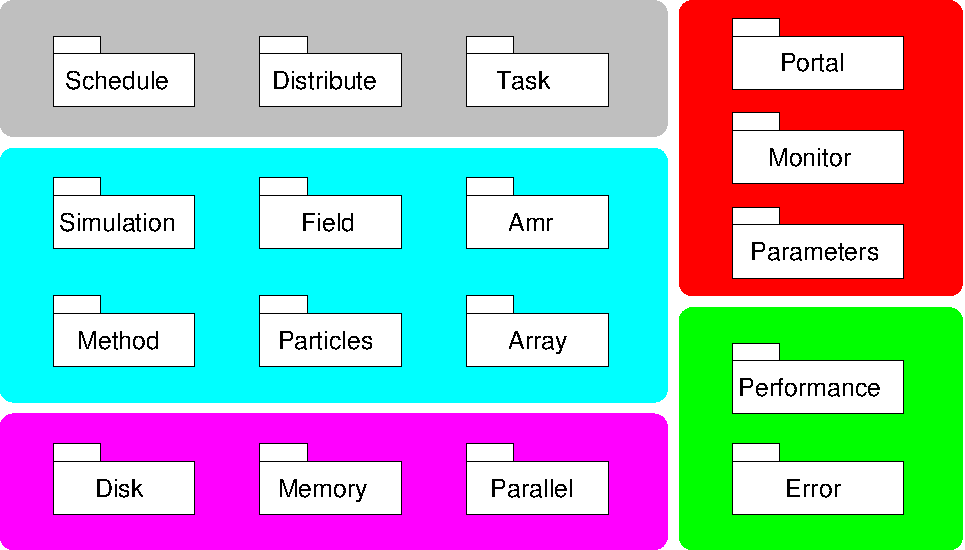
\includegraphics[width=3in]{components2.pdf}
\end{minipage}}

% \FIGURE{Software component diagram}{f:components}{
% \begin{minipage}{6in}
% 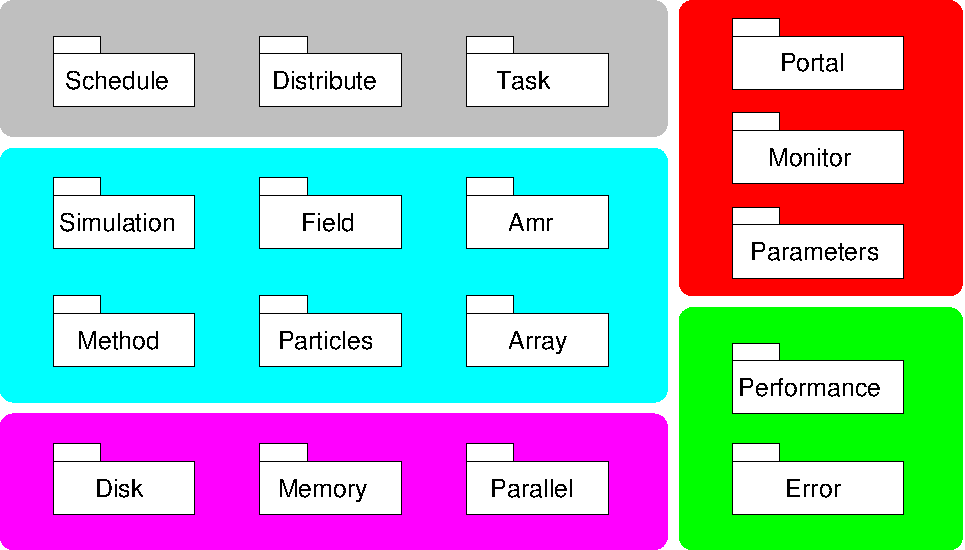
\includegraphics[width=6in]{components2.pdf}
% \end{minipage}}

The high-level components include \code{Task} for encapsulating
parallel tasks, \code{Distribute} for distributing and load balancing
tasks across available resources, and \code{Schedule} for scheduling
the tasks for execution.

The middle-level components include \code{Simulation} for defining the
simulation, and \code{Method} for user functions for
performing the numerical computations, inline analysis, and
visualization processing required to run the simulation.  Distributed
AMR is implemented in the \code{Amr} package, with related components
\code{Field} and \code{Particles} for representing data fields and
particle groups defined on the AMR hierarchy.  \code{Array} is a
component for defining and manipulating distributed Fortran-like
arrays.

The low-level components include API's for interacting with hardware,
including \code{Disk} for disk I/O, \code{Memory} for dynamic memory
management, and \code{Parallel} for parallel synchronization and data
transfer.  Including these lower level components is helpful for
several reasions: it encapsulates lower-level library calls, e.g.~HDF5
for \code{Disk}, which can include extra functions for collecting
performance data; it allows for incorporating error checking code,
e.g.~ tracking memory usage and performing bounds checking in
\code{Memory}; and parallel technologies such as MPI, UPC, and OpenMP
can be encapsulated in \code{Parallel}.

Components implementing cross-cutting concerns include
\code{Parameters} for reading, storing, and accessing parameters,
\code{Monitor} for logging performance and status information, and
\code{Portal} for dynamically interacting with external utilities or
systems.  \code{Performance} is used for collecting and accessing
performance-related data, and \code{Error} is used for signalling
hardware or software faults.

Component sizes will vary: \code{Amr} is expected to be large since
representing and manipulating distributed AMR hierarchies is
inherently complex, whereas \code{Memory} is likely to be relatively
small.  Larger components will be further decomposed into smaller
sub-components, e.g.~\code{Amr} may contain \code{Tree}, \code{Patch},
\code{Level}, and \code{Box} subcomponents, to help organize and
control software complexity.  Larger components may be implemented
using several interacting class hierarchies, whereas smaller
components may be implemented as a single class.

Below in sections \S\ref{ss:design-amr} through
\S\ref{ss:design-resilience} we describe preliminary design issues
related to requirements listed in sections \S\ref{ss:require-amr}
through \S\ref{ss:require-resilience}, respectively.

%-----------------------------------------------------------------------
\subsection{Adaptive mesh refinement} \label{ss:design-amr}
%-----------------------------------------------------------------------

How adaptive mesh refinement is designed is crucial for it to meet the
scaling requirements outlined in \ref{ss:require-amr}.  It must
maintain high parallel efficiency throughout the range of single-level
``unigrid'' problems, through ``wide'' problems requiring millions of
patches, and ``deep'' problems requiring several dozens of levels.
All must be efficiently mapped to HPC architectures with millions of
cores with fixed physical memory capacity per node.

The most important AMR data structure design decision is what variant
of AMR to use.  The two leading variants are ``block-structured AMR
(SAMR)'', or patch-based AMR, as used by \samrai\ and \chombo; and
``continuous AMR (CAMR)'', or octree-based AMR, as used by \paramesh.
There are numerous advantages and disadvantages to each, and
significant effort has gone into deciding which approach to pursue.
We have decided on a modified octree-based AMR approach, with two
modifications that improve AMR efficiency for both ``wide'' and
``deep'' problems.  We review these two modifications below.

We feel that octree-based approaches are arguably more
scalable~\cite{BuGh08}, in part because they avoid the parallel patch
placement algorithms required by SAMR, which are a significant
hinderance to scalability~\cite{GuWi06}.  Also, high quality SAMR
frameworks such as \chombo\ and \samrai\ are already available and
being actively developed.  Lastly, the octree in octree-based AMR can
be leveraged for particle neighbor searches; octrees have particularly
efficient representations and operations~\cite{FrPe02}; and absolute patch
extents are computed not stored, which can be used to address
precision and range issues of global indices that arise for extremely
large or deep AMR hierarchies.

Standard octree-based approaches involve either an octree or a forest
of octrees.  Nodes of the octree typically correspond to small
fixed-size locally-Cartesian grid blocks, such as the $4^3$ grid
blocks used in the FLASH astrophysics application built on the
\paramesh\ framework.  Refining a tree node involves partitioning the
node into eight octants, and coarsening involves the inverse
operation.  Mesh blocks can be associated with either all nodes in the
tree, or just the leaf nodes.  If the tree supports particle data as
well, particles are generally associated with leaf nodes.  To
eliminate ``level jumps''---a maximum of one level difference between
adjacent mesh blocks---a ``balancing'' operation is performed by
refining all coarse blocks that are adjacent to blocks that are
greater than one level finer.  Time steps are globally determined,
but may be adaptive at each resolution level.

Parallelizing involves distributing $N$ tree nodes across $P$
processors.  This is frequently accomplished using a space-filling
curve: first blocks are linearizing using a linearized Morton, Gray
code, or Hilbert ordering; then the list is divided evenly into $P$
section, with blocks in the $k$th section assigned to the $k$th
processor.

There are several operations required of the distributed AMR data
structure, all of which must be designed and implemented in a highly
scalable manner.  These include generating the initial grid hierarchy,
dynamically refining and coarsening grid patches or blocks,
maintaining a balanced AMR data structure free of level jumps,
defining and distributing parallel computational tasks, and
maintaining a uniform work distribution by dynamically load balancing
tasks.  The AMR data structure must also support efficient access to
grid block/patch mesh data and particles.  This includes interpolating
data between hierarchy levels, and accessing mesh data and particles
in adjacent blocks, which is required for computational stencils and
locality-depedent particle methods such as $P^3M$.

As described, there are several issues with the standard octree-based
AMR approach that we wish to address.  
%
1) By only supporting small fixed-sized blocks, the AMR data structure
size can grow very large in reqions in which the resolution is
uniform.
%
2) The AMR data structure can also grow large for ``deep'' AMR
problems due to the combination of the shallow refinement-by-two and
octree balancing steps.
%
3) Extremely deep AMR runs can consume a large amount of memory
relative to the small amount of available parallelism, making them
unrunable on machines that have restricted memory per process.
%
4) For extremely large or extremely deep AMR problems, the excessive
range of global indices, or excessive precision of particle positions,
can require 64-bit or higher integers / floats.
%
5) Determining the time step generally requires global reduction
operations, which we wish to avoid if possible for scalability.
%
6) Applications frequently store the hierarchy ``metadata''---the AMR
data structure excluding mesh and particle data---redundantly on each
processor, which is a roadblock to scalability.

We summarize our approaches to these issues below.  Two more
fundamental issues, parallelism and load balancing, are described in
their own sections \S\ref{ss:design-parallel} and
\S\ref{ss:design-balance}, respectively.

%------------------------------------------------------------------------

\textbf{1) Patch coalescing.} One proposed enhancement to the typical
octree-based AMR approach is to allow variable mesh sizes per AMR
hierarchy patch.  This can be introduced using the simple invertable
AMR-invariant operation illustrated in Figure~\ref{f:coalesce}.  While
keeping the underlying mesh resolution constant, the operation
transforms multiple AMR patches with a single patch, but with a larger
mesh.  We call this \textit{patch coalescing}.  The inverse operation
is permitted as well if the patch requires subsequent refinement or
coarsening.

\FIGURETWOCOL{Coalescing}{f:coalesce}{
\begin{minipage}{1.875in}
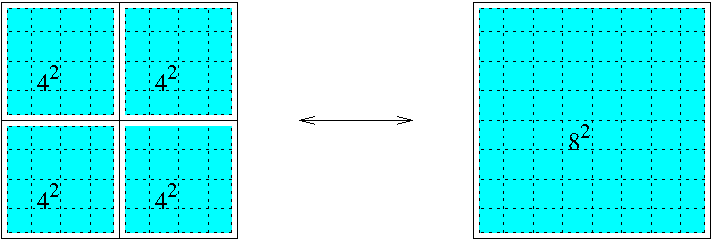
\includegraphics[width=1.875in]{coalesce.pdf}
\end{minipage}}

% \FIGURE{Coalescing}{f:coalesce}{
% \begin{minipage}{3.75in}
% 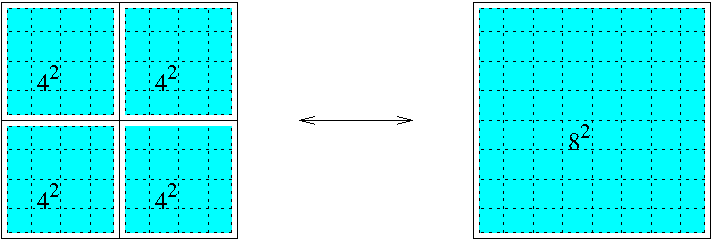
\includegraphics[width=3.75in]{coalesce.pdf}
% \end{minipage}}


This operation decouples the AMR topology from the local resolution
requirements, which permits a more efficient AMR data structure for
the same resolution requirement.  Patch coalescing will be
particularly efficient for AMR problems that involve large regions
in which the resolution is uniform.  We note that this modification
is not relevant to block-structured AMR, since patch sizes are already
variable.

As a proof-of-concept, below in Figure~\ref{f:cosmo} is an image of a
2D cosmology density field projection, together with two balanced 2D
quadtrees adapted to the image's gray scale.  One of the quadtrees
used fixed-resolution patches, whereas the other used patch
coalescing.  Even though the example problem is not particularly
well-suited for this technique, it nevertheless leads to a quadtree
with $2 1/2$ times fewer nodes.

\FIGURETWOCOL{ Coalesced patches proof-of-concept using a 2D cosmology
  density field projection.  \textbf{Left}: 2D cosmology density field
  projection.  \textbf{Middle}: Balanced quadtree with 81701 patches.
  \textbf{Right}: Balanced quadtree with 32529 coalesced patches. \\
} {f:cosmo}{
\begin{minipage}{3.2in}
\begin{minipage}{1.0in}
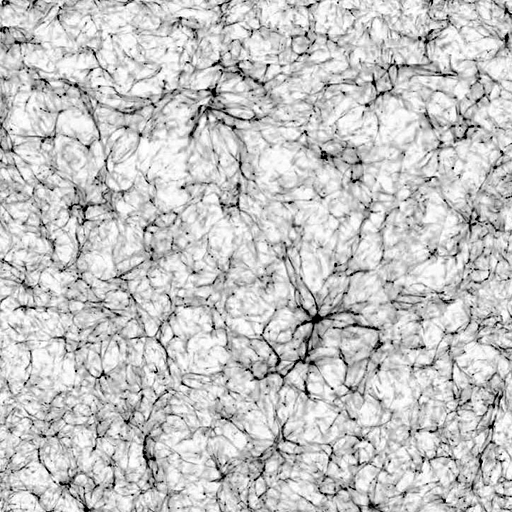
\includegraphics[width=1.0in]{cosmo2-invert.png}
\end{minipage} \ 
\begin{minipage}{1.0in}
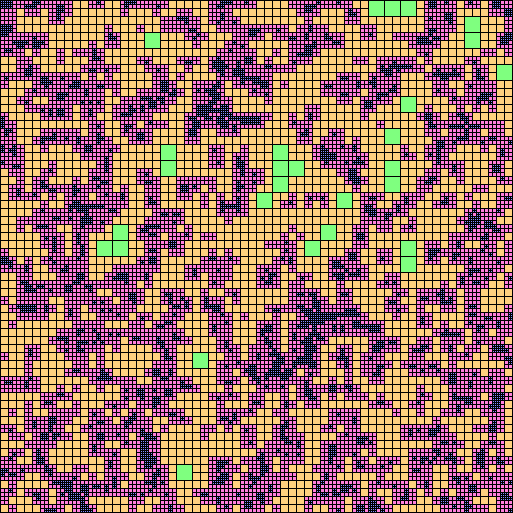
\includegraphics[width=1.0in]{cosmo2-4-1-inv.png}
\end{minipage} \ 
\begin{minipage}{1.0in}
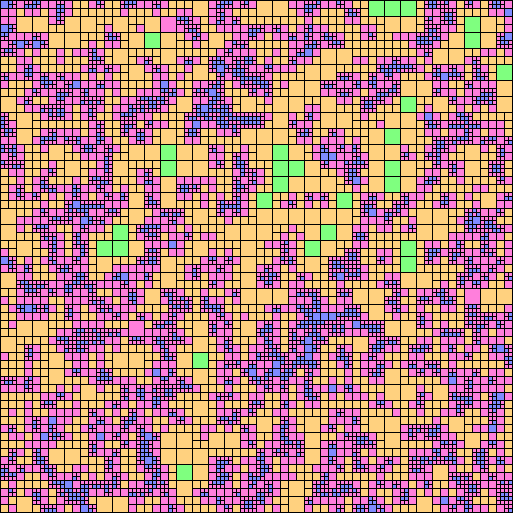
\includegraphics[width=1.0in]{cosmo2-4-2-inv.png}
\end{minipage}
\end{minipage}
}

% \FIGURE{ Coalesced patches proof-of-concept using a 2D cosmology
%   density field projection.  \textbf{Left}: 2D cosmology density field
%   projection.  \textbf{Middle}: Balanced quadtree with 81701 patches.
%   \textbf{Right}: Balanced quadtree with 32529 coalesced patches. \\
% } {f:cosmo}{
% \begin{minipage}{7.0in}
% \begin{minipage}{2.2in}
% 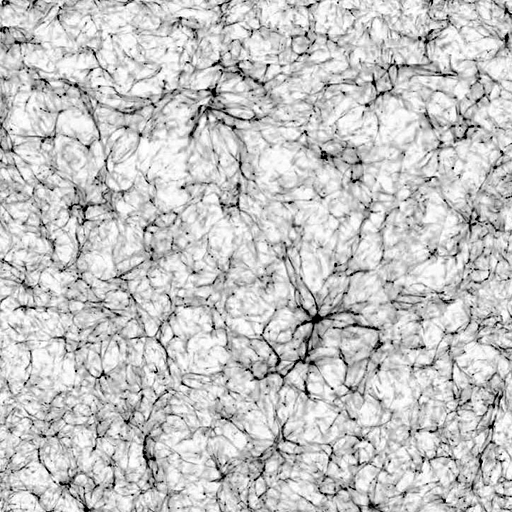
\includegraphics[width=2.2in]{cosmo2-invert.png}
% \end{minipage} \ 
% \begin{minipage}{2.2in}
% 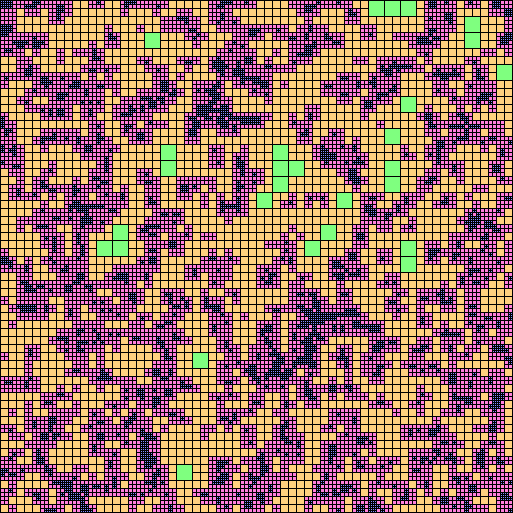
\includegraphics[width=2.2in]{cosmo2-4-1-inv.png}
% \end{minipage} \ 
% \begin{minipage}{2.2in}
% 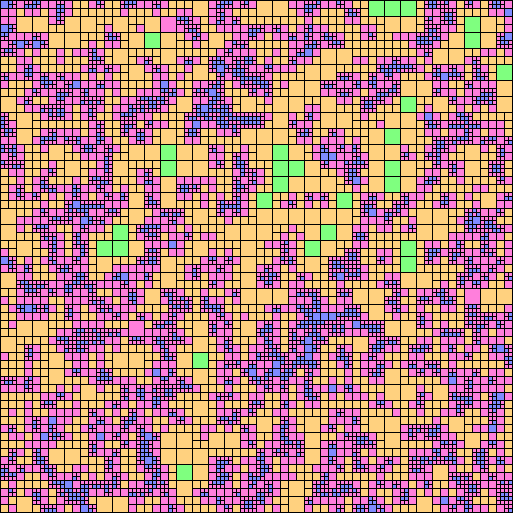
\includegraphics[width=2.2in]{cosmo2-4-2-inv.png}
% \end{minipage}
% \end{minipage}
% }

While allowing flexible patch block sizes can greatly reduce the size
of the octree-based AMR data structure, the variable block size can
complicate other issues, specifically load balancing and parallel task
definition.  Load balancing is complicated since work load per grid
patch is no longer ``constant'' within a level (though we argue later
that it is not necessarily constant to begin with), and task
definition is complicated by the wide variation in task size.  We
address this issue by decoupling parallel tasks from AMR patch blocks,
essentially by allowing parallelism within a patch block.  With this
approach, which we describe in more detail in
\S\ref{ss:design-parallel}, we can maintain a constant or bounded
subblock task size despite permitting arbitrarily large AMR patch
blocks.


%------------------------------------------------------------------------

\textbf{2) Targeted refinement.}  Another proposed enhancement to the
octree-based AMR approach is, instead of using a $2^3$-tree (octree)
and refining by $r=2$, we use a $4^3$-tree and refine by $r=4$, or an
$8^3$-tree and refine by $r=8$.  We call this $r^3$-tree approach
\textit{targeted refinement}.

The motivation and main advantage of targeted refinement is for
particularly deep AMR runs, where the region of interest is tiny
relative to the global domain size, such as simulations of galaxy or
star formation.  As a proof-of-concept example, in Figure~\ref{f:dots}
two balanced $r^2$-trees are shown refined on a small set of points in 2D, one
with $r=2$ and one with $r=4$.

\FIGURETWOCOL{
Targeted refinement proof-of-concept using multiple point sources in 2D.
\textbf{Left}: 2D point sources.  
\textbf{Middle}: Balanced octree with 2137 patches.
\textbf{Right}: Balanced octree with 158 explicit patches.
}
{f:dots}{
\begin{minipage}{3.2in}
\begin{minipage}{1.0in}
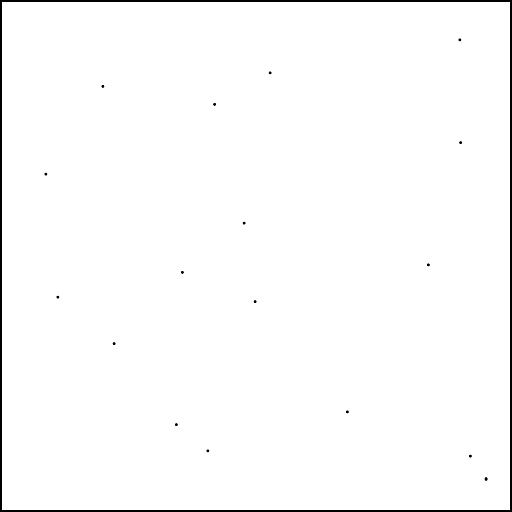
\includegraphics[width=1.0in]{dots-invert.png}
\end{minipage} \ 
\begin{minipage}{1.0in}
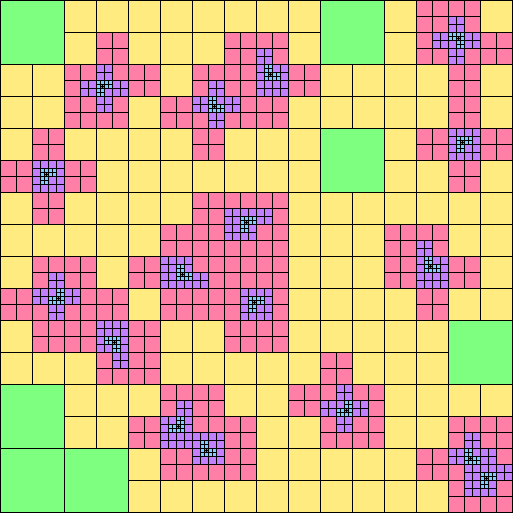
\includegraphics[width=1.0in]{dots-4-1-inv.png}
\end{minipage} \ 
\begin{minipage}{1.0in}
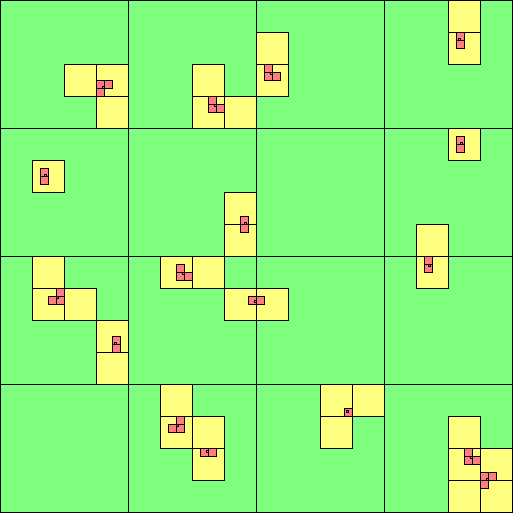
\includegraphics[width=1.0in]{dots-16-5-inv.png}
\end{minipage}
\end{minipage}}

% \FIGURE{
% Targeted refinement proof-of-concept using multiple point sources in 2D.
% \textbf{Left}: 2D point sources.  
% \textbf{Middle}: Balanced octree with 2137 patches.
% \textbf{Right}: Balanced octree with 158 explicit patches.
% }
% {f:dots}{
% \begin{minipage}{7.0in}
% \begin{minipage}{2.2in}
% 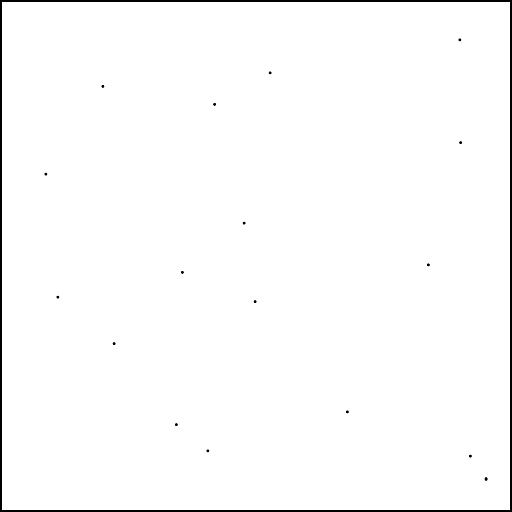
\includegraphics[width=2.2in]{dots-invert.png}
% \end{minipage} \ 
% \begin{minipage}{2.2in}
% 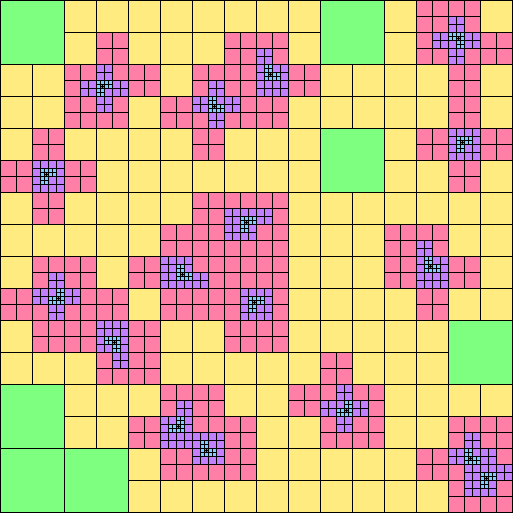
\includegraphics[width=2.2in]{dots-4-1-inv.png}
% \end{minipage} \ 
% \begin{minipage}{2.2in}
% 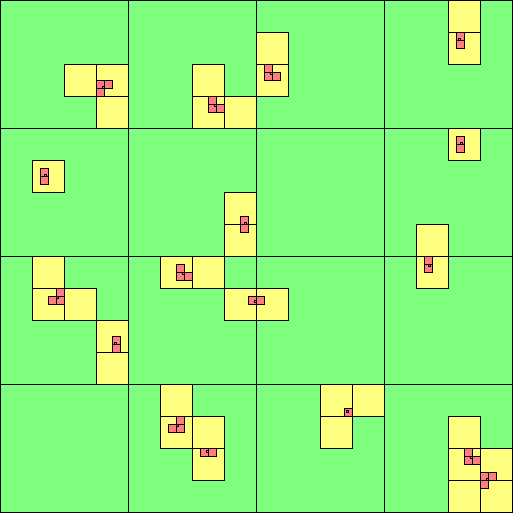
\includegraphics[width=2.2in]{dots-16-5-inv.png}
% \end{minipage}
% \end{minipage}}

The advantage is clear: the number of nodes in the AMR hierarchy is
reduced by a factor of about $13.5$.  There are apparent disadvantages
as well.

One disadvantage is that balancing an $r^3$-tree still allows jumps in
refinement greater than two.  We can regain this mesh constraint by
introducing implicit \textit{backfill} patches, as indicated in
Figure~\ref{f:backfill}.

\FIGURETWOCOL{Targeted refinement with backfill}{f:backfill}{
\begin{minipage}{3in}
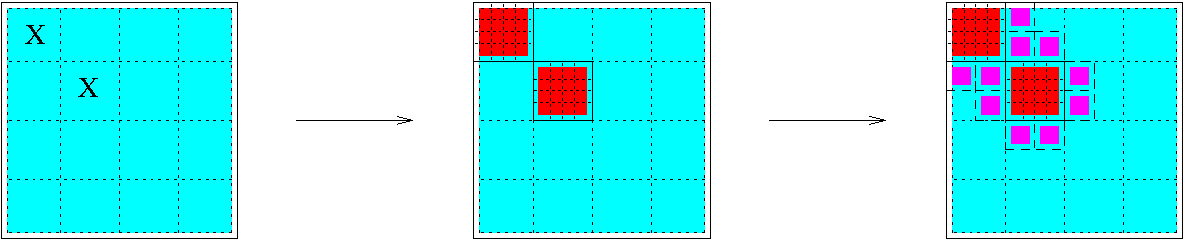
\includegraphics[width=3in]{kd-backfill.pdf}
\end{minipage}}

% \FIGURE{Targeted refinement with backfill}{f:backfill}{
% \begin{minipage}{6.15in}
% 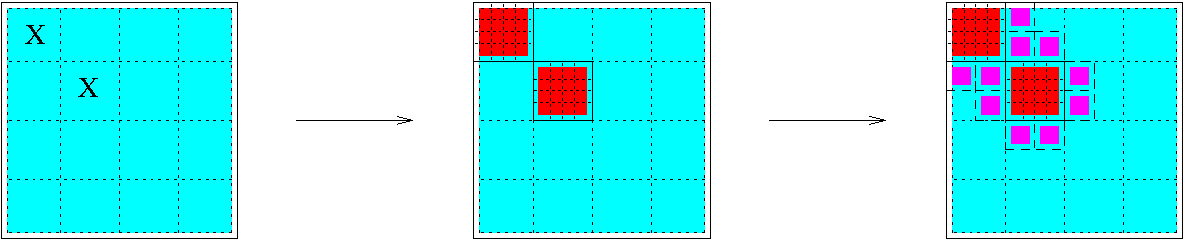
\includegraphics[width=6.15in]{kd-backfill.pdf}
% \end{minipage}}

Another disadvantage is that we need to represent the $r^3$-trees.
This can be done by simply using the $2^3$-tree data structure
implementation and ignoring intermediate levels.  This still reduces
the overall data structure size, since the balancing step is only
performed on the ``active'' levels.  This can also improve parallel
scaling: the $2^3$-tree balancing operation potentially affects all
levels of the hierarchy,.whereas for $r>2$ the $r^3$-tree balancing
and backfill operations are more localized.

%------------------------------------------------------------------------

\textbf{3) Level window.}  For particularly deep AMR runs, the
amount of parallelism is relatively small, since the serial bottleneck
is the time step on the finest levels.  Memory consumption can be
large, however, especially relative to the amount of parallelism.
These problems stress scaling not just due to the limited parallelism
available, but because of restriced amount of physical memory
available per process.

We plan to address this issue not just by increasing parallelism, but
by reducing the memory requirement per process by deallocating
unnecessary storage.  Because of the smaller time steps taken on finer
levels, the simulated time of interest can be much less than the time
steps at the coarser levels.  If it is known that data at a coarse
level is no longer required, then that level can simply be removed
from the simulation, freeing up resources for finer levels.  In
principle, this could allow arbitarily deep AMR runs, since only a
fixed interval or ``window'' of levels may be required.  This would
only be feasible if other data structure limits and numerical scaling
is handled appropriately, and provided the total number of fine level
time steps is not excessive.

%------------------------------------------------------------------------
\textbf{4) Implicit global indices.}  For particularly large and deep
AMR runs, the range of global indices and precision of absolute
positions can become issues.  The limits of 32-bit values can quickly
be exhausted, and it is conceivable that for extreme AMR even 64-bit
values is insufficient.  This can lead to increased memory usage for
storing the AMR meta-data, and increased code complexity to support
non-standard 128-bit values.

Our approach will be to support the option of not storing global
indices and positions for the supporting AMR data structure, and only
compute them when absolutely necessary.  The octree data structure
defines the relative configuration of a block with its parent,
neighbors, and child blocks, which is sufficient for many operations.
In particular, only knowing the local mesh width and timestep is
sufficient for many hyperbolic conservation problems.

Some operations may require absolute positions however, such as
problem initialization, inline analysis routines, or internal material
boundaries.  In these cases absolute positions or indices can still be
determined using the octree data structure in $O(\log N)$ time, using
whatever precision or range is necessary.  A similar approach for
particle positions is outlined in \S\ref{ss:design-particles}.


%------------------------------------------------------------------------

\textbf{5) Patch-local adaptive time steps.} There are two common
variants in time step determination: uniform time steps over the
entire domain, and adaptive time steps at each refinement level.
These variants have their relative advantages and disadvantages:
adaptive time steps are more computationally efficient, especially for
``deep'' AMR runs, whereas using uniform time steps is more scalable
since all patches can advance a time step simultaneously.

One disadvantage of both is that determining the time step, either for
the entire domain or within individual levels, requires a global
reduction operation.  However, global operations are particularly costly for
massively parallel machines.  

We believe this global operation can be avoided by relaxing the
constraint of a fixed time step within a level.  The time step is
determined to a large part by the spacial resolution of the mesh,
which is constant within a level; however, in highly dynamic regions
such as rapid gravitational collapse, the local physics may lead to
requiring a smaller time step.  Instead of allowing these isolated
regions to determine the time step for the entire level, we will
optionally permit individual patches to make multiple time steps
relative to other patches in the same level.  For some problems, this
may help prevent rapidly evolving feature in one localized region of
the domain from determining the time step everywhere else.


%------------------------------------------------------------------------

\textbf{6) Distributed data structure.} There are two main approaches
used for representing the AMR hierarchy structure on a distributed
memory machine: storing part of the hierarchy on each process, and
storing the entire hierarchy on all nodes or processes.

Each clearly has its advantages and disadvantages.  Duplicating the
entire hierarchy on all processes can be more efficient, since
operations involving the hierarchy as a whole may require no
communication.  Storage of octree data structures is extremely
efficient, using at most three pointer variables~\cite{FrPe02}.  However,
the approach still ultimately does not scale, because it requires
$O(N)$ storage and computation per process, and since available memory
per process is always limited.  As the problem size grows, eventually
the AMR data structure storage will exhaust all available physical
memory.

Our solution, which has been used by others
(e.g.~\cite{@@@hybrid-storage}), will be to support a hybrid
duplicated and distributed AMR data structure.  Coarser levels, which
span wider areas of the domain, can be stored redundantly but
efficiently on every process.  Grid patches in finer levels (along
with a layer of adjacent ``remote proxy patches'' analagous to ghost
zones for AMR patches) can be stored only on the local processes to
which the patches are assigned.  The exact level at which the switch
occurs may be arbitrary, may change during a simulation, and may vary
in different regions of the domain, depending on how the local tradeoff
between memory and communication costs change.

In the following two sections, we describe our treatment of mesh data
and particle data.

%-----------------------------------------------------------------------
\subsection{Mesh data} \label{ss:design-fields}
%-----------------------------------------------------------------------

Mesh data, as described previously, will be represented as locally
Cartesian grids on octree nodes.  The stored size may vary, but the
parallel task size may be kept constant, which implies that field data
in a single patch may be distributed across multiple processes.  In
the limit of a large ``unigrid'' (single AMR level) run, the AMR data
structure would be a single octree node, and the array would be
partitioned into at least $P$ blocks.

As outlined in the mesh data requirements
section~\S\ref{ss:require-fields}, there will be any number of
user-defined fields, which may be stored using either single or double
precision.  Different fields are identified by user code using 
opaque field ID's, and by users (e.g.~in output files) by
user-defined string identifiers.  Different user methods may
declare different fields to be read-only, or writable.

Optional scaling factors may be defined, which may vary for different
fields, different AMR levels, or different methods.  Level-dependent
scaling factors may be defined if the user's solvers have
scale-sensitive numerical behavior, and method-dependent scaling
factors may be defined to simplify the integration of different
solvers that expect fields to be stored using different physical
units.

Ghost zone data may be either explicitly stored, or only allocated
when required.  Ghost zone depths may vary between fields to improve
memory utilization and the cost of copying data that is not required
by the user's solvers.  

Users may optionally specify bounds on individual fields, e.g. a
minimum of $0$ or some small positive constant for pressure.  This
will allow \cello\ to optionally check for some software or numerical
errors.  If a field goes out of bounds, then some action can be taken
to address the problem, such as reduce the size of the time step
constraint or switch to an alternate solver.  Support for more general
assertions on field values may be implemented as well, such as checking
that conserved fields are indeed conserved, or similar constraints
such as $\nabla\cdot B=0$ for MHD problems.

%-----------------------------------------------------------------------
\subsection{Particle data} \label{ss:design-particles}
%-----------------------------------------------------------------------

The same octree data structure that is used to support
multi-resolution field data will also be used to spacially organize
particles.  Particles will be associated with leaf nodes of the
octree, which will enable fast and accurate Lagrangian methods such
as $PPPM$~\cite{HoEa88}.

Particles will also be grouped into arbitrary user-defined particle
groups.  As indicated by the requirement summary, different particle
groups may have arbitary user-defined logical, integer, or
floating-point attributes associated with each particle in the group.
Particle groups are identified by user code using opaque particle
group ID's, and by users by user-defined stringe identifiers.

To address the issue of AMR depth-dependent precision requirements on
global particle positions, particle positions may optionally be stored
relative to a local coordinate system defined by the containing AMR
patch.  This is illustrated in Figure~\ref{f:local-particles}.  One
advantage is that for very deep AMR levels, the accuracy of
patch-local positions do not deteriorate due to catastrophic
cancellation, as they do when global positions are stored.  Also, even
single precision is expected to provide more than sufficient
positional accuracy for local computations, which will additionally
improve both memory storage requirements and memory access costs.

\FIGURETWOCOL{Patch-local coordinate systems for
  particles}{f:local-particles}{
\begin{minipage}{3.2in}
\begin{minipage}{1.5in}
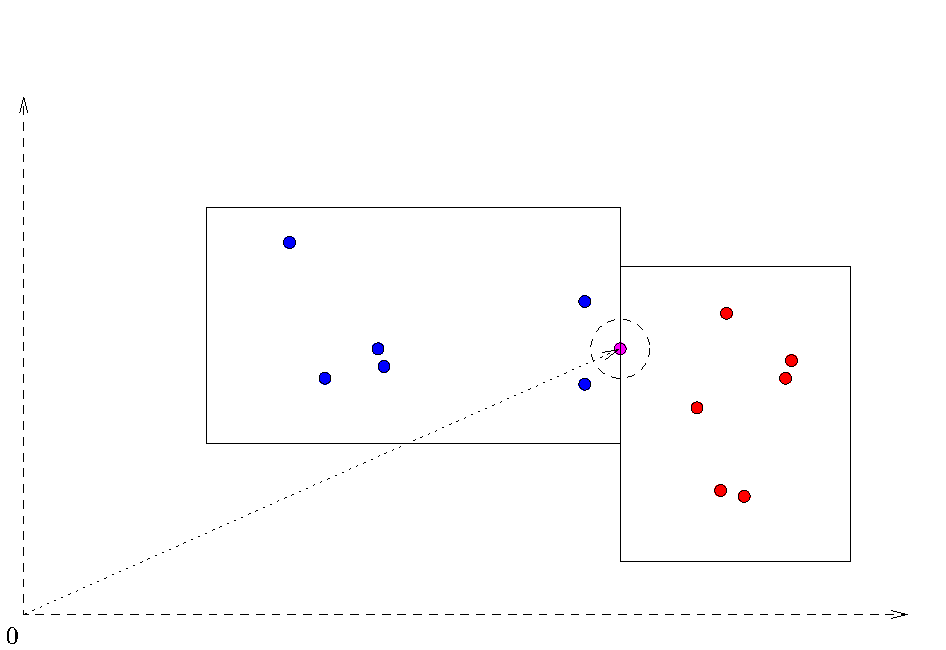
\includegraphics[width=1.5in]{particles-global.pdf}
\end{minipage} \ 
\begin{minipage}{1.5in}
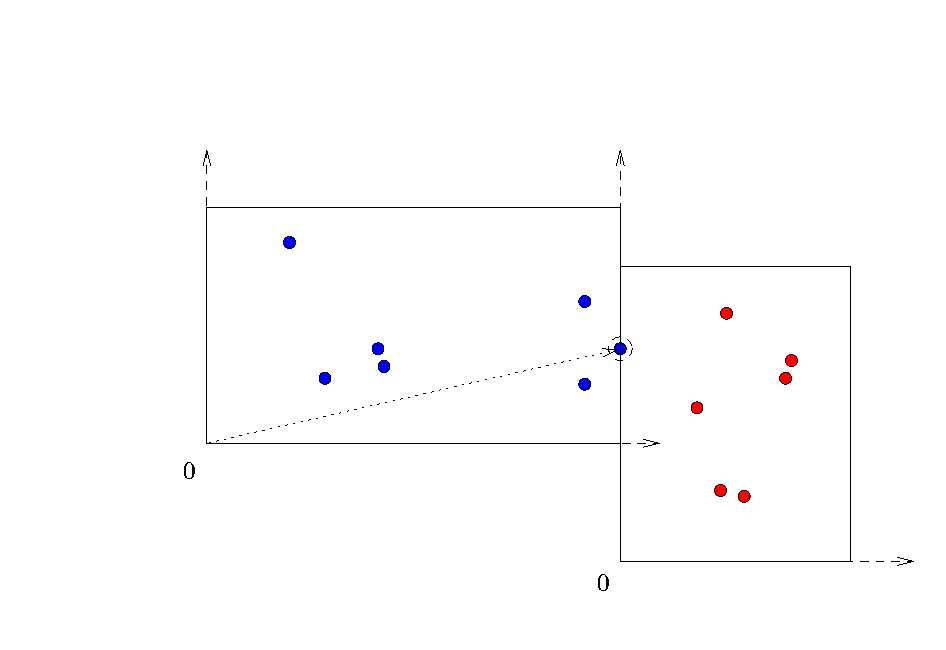
\includegraphics[width=1.5in]{particles-local.pdf}
\end{minipage}
\end{minipage}}

% \FIGURE{Patch-local coordinate systems for
%   particles}{f:local-particles}{
% \begin{minipage}{6.8in}
% \begin{minipage}{3.3in}
% 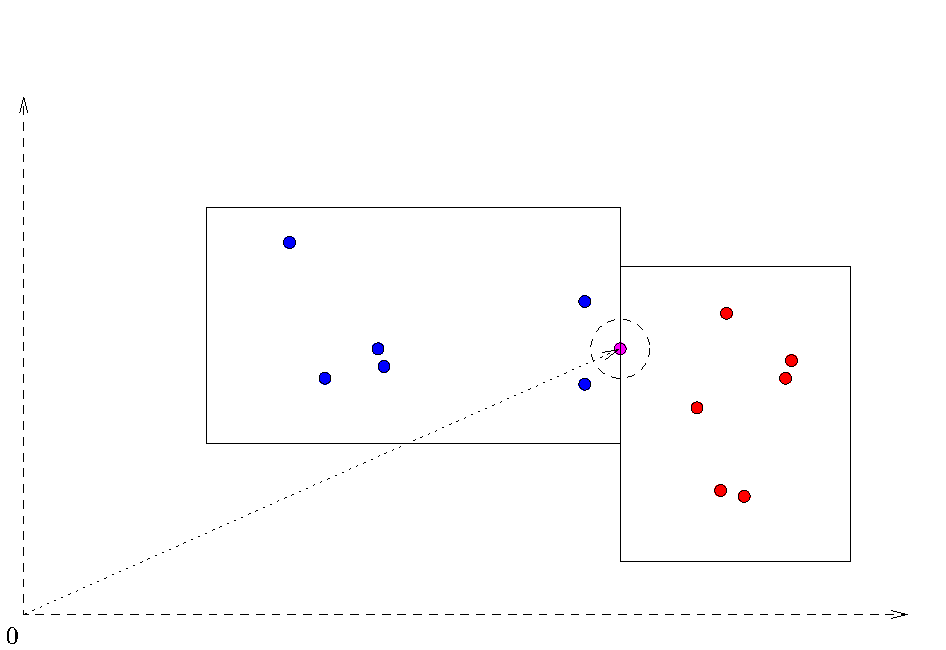
\includegraphics[width=3.3in]{particles-global.pdf}
% \end{minipage} \ 
% \begin{minipage}{3.3in}
% 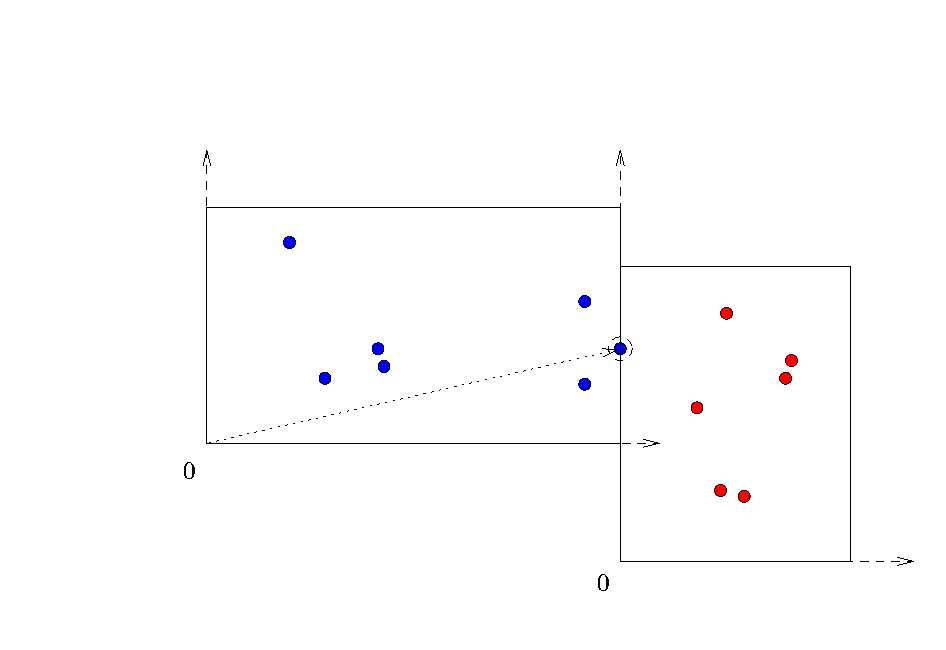
\includegraphics[width=3.3in]{particles-local.pdf}
% \end{minipage}
% \end{minipage}}

A consequence of using patch-local coordinate systems is that
particles that relocate from one patch to a neighboring patch will
require a coordinate transform: this transformation is trivial to
implement and compute.  Also, sometimes global particle positions are
still required, for example for analysis or visualization.  In these
cases global positions can still be made available by providing
functions for accessing global as well as local particle positions.
Global positions can be internally computed by \cello\ to any required
precision by traversing the AMR octree with $O(\log N)$ cost, even
if they are not explicitly stored.

%-----------------------------------------------------------------------
\subsection{User functions} \label{ss:design-user}
%-----------------------------------------------------------------------

How user functions interface with \cello\ is an important design
issue, since it balances ease of use with power and flexibility.  

User initialization functions will be required to define the fields
are particle groups that will be used.  These functions may initialize
fields and particles as well, or simple initialization can be
performed using \cello\ parameter files.  Physics functions must also
be ``registered,'' which may involve declaring which field or particle
groups are read or modified by each function, whether each function is
patch-, level-, or hierarchy-oriented, whether a method requires
either temporary or persistent local fields or particle groups, and
how functions are to be sequenced.  Initialization functions also
assign string identifiers by the user, which is used for example to
support user function-specific run-time parameters.  To improve
software resilience, alternate methods may also be specified, which
\cello\ will invoke in the event the primary method signals a failure.

The primary physics-related user functions will be those that advance
the field or particle data one timestep on a single logically
Cartesian grid.  \cello\ will schedule and execute these user
functions on individual patch blocks as outlined in
\S\ref{ss:design-parallel}.  

The secondary physics-related user functions will be for computations
at level interfaces, such as flux-correction or other constraint
enforcement at AMR level boundaries.  In this case user code will
operate on fields and particle data defined on two adjacent patches in
different levels, rather than a single patch.  Scheduling and
executing these functions will also be controlled by \cello's scheduler.

Other user-functions supplied will be AMR-related, and include tagging
AMR patches for refinement or coarsening, and determining the local
time step.

All user functions will have access to \cello\ API's, which include
signalling a software or method failure, defining additional
values for user monitoring during a running simulation, and for
measuring performance.

%-----------------------------------------------------------------------
\subsection{Run-time parameters} \label{ss:design-parameters}
%-----------------------------------------------------------------------

The run-time parameters component will use \code{flex} and
\code{bison} parsing tools to generate code to read and parse the
run-time parameter file.  Parameter types will include integers,
scalars, logicals, strings, and lists.  Logical and scalar expressions
involving spacial variables \code{x}, \code{y}, and \code{z}, and time
variable \code{t}, will also be supported to enable defining simple
initial conditions and time-dependent boundary conditions via the
run-time parameter file.

The run-time parameters API will allow access to parameter values by
type, as well as evaluation of scalar and logical expressions
involving \code{x}, \code{y}, \code{z}, and \code{t}.  User-defined
parameters can be accessed by user code, so that parameters specific
to the user code can be integrated into the same run-time parameters
file as the \cello\ parameters.  Related parameters will be grouped
into individual sections, e.g.~fields, particles, AMR, user functions,
etc., to improve organization of the parameters.

%-----------------------------------------------------------------------
\subsection{Parallelism} \label{ss:design-parallel}
%-----------------------------------------------------------------------

For a hyperpolic problem defined on an arbitrary AMR hierarchy, any
given patch in the hierarchy may advance one time step if all of its
boundary data is up to date.  Assuming that the advancement of a grid
patch one time step is taken to be a parallel task, this defines a
dependency graph.  \cello\ will use this dependency graph to control
the parallel execution of the simulation.

Since the AMR approach will include varying patch sizes, data on a
single patch may be distributed among multiple processes.  The basic
approach of defining a dependency graph will still be used, but
sub-patches will be used to define a parallel task.  In \cello, a task
may be an entire patch, or a portion of a patch.  Task sizes can be
controlled by restricting sub-patch sizes within a given range, which
may be constant.  Tasks are encapsulated in the \code{Task} software
component.

\cello\ will maintain a priority queue of runnable tasks on each
process.  Such dynamic scheduling is well suited for heterogeneous
sized tasks and non-regular communication dependencies. Tasks
associated with sub-patches in finer AMR levels will likely be given
higher priority since they determine the critical path through the
dependency graph.  Communication will be similarly scheduled to
effectively prefetch ghost data required by a patch so that it is
available when the patch is executed.  Scheduling and execution of
tasks will be controlled by the \code{Schedule} software component.

Execution of tasks and communication of ghost data will be performed
using ``computational registers'' (motivated by and analagous to
``working block'' or ``work'' data structures in \paramesh), and
``flux registers'' (motivated by and analagous to
\code{LevelFluxRegister}s in \chombo).  This overall approach will
allow decoupling of how data is stored in the AMR data structure from
how it is stored when it is being actively computed or communicated.
This in turn permits flexibility to 1) optimize how data is stored
when not being processed, e.g.~without ghost zone data to greatly
reduce memory use, 2) optimize how data is stored when it \textit{is}
being processed, either to ease the interface to user code or to
rearrange data to improve cache performance when being processed, and
3) optimize how ghost zone data is communicated, e.g.~to group
multiple communication requests between a pair of processes or nodes
together into a single communication call to improve communication
performance.

This overall task approach maps well to the data-driven process
virtualization model used by \charm, the functionality of which
subsumes that of both the \code{Task} (``chare'') and \code{Schedule}
components, as well as \code{Distribute}, which is used for task
distribution and dynamic load balancing (\S\ref{ss:design-balance}).  This
similarity is no coincidence, since the \charm\ model helped influence
our high-level parallelization design.  \charm\ also \charm\ also
provides fault tolerance support through its built-in disk, or memory
+ disk, checkpoint / restart mechanism.  Because of this close match
in design, we will begin parallel development using the high-level
\charm\ framework.

However, later development will also include supporting message
passing via the MPI library~\cite{wwwmpi}, partitioned global address
space (PGAS) programming via the UPC
language~\cite{wwwupc}~\cite{upc}, and shared memory parallel
programming via OpenMP API~\cite{wwwopenmp}.  We will also allow
direct support of hybrid parallelism approaches, including MPI with
OpenMP, and MPI with UPC.

There are several other reasons why we plan to include multiple
parallelization technologies.  First, because the performance and
scalability of the technologies vary between machines and
implementations~\cite{MaTa09}, and we want to always use the fastest
and most scalable approach.  Second, one technology may perform better
in the distributed memory regime, whereas another may perform better
within a shared memory node, which motivates flexible hybrid parallel
approaches.  Third, by including multiple existing parallelization
paradigms from the start, we expect that the resulting software design
will be more amenable to incorporating new parallelization
technologies that may be developed in the future.  And fourth, the
framework could be used as a benchmark tool for parallel technology
designers to evaluate their approaches (\cite{WeSu07}).

The low level \code{Parallel} component will encapsulate the core
parallel synchronization and data transfer operations, which will
remove dependencies on MPI, UPC, or OpenMP from other components.  We
expect the \code{Parallel} component will include two parallelization
API's, one for distributed memory and one for shared memory; the
distributed memory API would encapsulate MPI and UPC, whereas the
shared memory API would encapsulate OpenMP and UPC.  The
\code{Parallel} component will also directly support hierarchical
parallelism, which we will use to improve the mapping of data and
communication onto the specific hardware, for example hierarchical
load balancing summarized in \ref{ss:design-balance}.  Additionally,
while heterogeneous platforms such as those containing general purpose
graphics processing units (GPGPU's) will not be directly supported,
the framework's design will facilitate their use by user-written
physics kernels written for GPGPU's.

While the higher level \code{Schedule}, \code{Task}, and
\code{Distribute} components will be independent of whether MPI, UPC,
or OpenMP is used, it will still be dependent on whether \charm\ is
used.  We still expect to reuse much of the \charm-related code in the
higher level components when augmenting the code with other
parallelism technologies, such as functions for ``packing'' and
``unpacking'' task-related data required for task migration.  This
code reuse will help reduce development time.

%-----------------------------------------------------------------------
\subsection{Load balancing} \label{ss:design-balance}
%-----------------------------------------------------------------------

The \code{Distribute} component will be used to distribute and
dynamically load balance tasks across available computational
resources.  Dynamic load balancing is well known to be a crucial
operation for extreme scalability in general, and for extreme adaptive
mesh refinement in particular.  Computational load must be evenly
distributed to maintain high overall parallel computational
efficiency; dynamically allocated memory must be well-distributed
across compute nodes to avoid depleting available physical memory; and
data locality must be maintained within compute nodes to maintain high
communication performance over the interconnect.

\textbf{Space-filling curve approach.}
A common approach to distributing octree-based SAMR hierarchy tasks is
to linearize the data structure using a Morton, Gray code, or Hilbert
type space-filling curve, then partition the tree nodes among
processes by dividing the linearized structure into $N_P$ evenly sized
pieces.  This approach has been shown to scale to over $60K$
cores~\cite{@@@ART}, and works well if workload and memory usage are
proportional to each other within tree nodes, when workload between
tree nodes is roughly equal, and when the evolutionary change in the
hierarchy is sufficiently restricted.

However, we anticipate that this approach will not be sufficient for a
general-purpose extreme AMR framework for several reasons.
%
First, adaptive time steps are required for efficient ``deep'' AMR
problems, but that scales the work load for a given node by a
non-constant factor of roughly $2^k$ for level $k$.
%
Second, particle distributions among nodes may not be uniform, affecting both memory and computational loads.
%
Third, array patches may be differently sized, if we use our
``coalesced patches'' enhancement to reduce the AMR tree node count.
%
And fourth, performance of physics methods on a patch is not
necessarily uniform, e.g.~due to localized subcycling of stiff
methods, extra computations along shock fronts for front tracking
methods, etc.  
%The first three issues, and possibly the fourth, could
%be addressed by dynamically weighting nodes before partitioning them
%among processes, but that would require additional global
%communication to perform the reduction.
%
Also, this approach will eventually be unscalable since it
requires $O(N_P)$ storage per process, and a global all-gather
operation (e.g.~\code{MPI\_Allgather}) is required on all processes.

Since we suspect that a space-filling curve approach is only effective
for a strict subset of AMR problems we wish to support, we will also
explore two ideas for dynamic load balancing, including ``hierarchical
diffusion-based load balancing'', and a technique we call
``deliberate overcompensation''.

\textbf{Hierarchical diffusion-based approach.} Load balancing
schemes can be either global or local.  Global schemes, such as
space-filling curves or spectral methods, are considered to either
generate lower-quality task partitionings quickly, or produce
high-quality partitionings slowly~\cite{MeMo09}.  Local schemes,
such as diffusion-based methods, are considered to be efficient
at balancing tasks locally, but cannot effectively balance tasks
globally.

Due to the hierarchical nature of HPC platforms, we believe that a
hierarchical load balancing scheme will be the most effective approach
for both scalability and efficiency.  By \textit{hierarchical load
  balancing} we mean rebalancing tasks between higher levels (nodes or
supernodes) independently from rebalancing between lower levels
(socket or cores).  The idea of hierarchical task scheduling and load
balancing has been explored for at least 15 years~\cite{AhGh94}, and
is being actively adapted specifically to AMR
applications~\cite{LaTa06}, but is not commonly available in currently
existing AMR frameworks.

We will begin with a hierarchical load balancing scheme such as that
developed in~\cite{LaTa06} specifically for AMR applications.
Hierarchical load balancing will have several advantages over more
traditional non-hierarchical load balancing methods.  First,
rebalancing at different levels could be based on different metrics,
e.g.~memory usage together with computational load for rebalancing
between nodes, but just computational load for rebalancing between
processes or threads within node.  Balancing with respect to memory
across nodes will be particularly useful for AMR problems, because
memory is the crucial metric we want to keep balanced at the node
level, yet we want to balance computational time at lower hardware
platform levels to keep computational elements busy.  Second,
hierarchical load balancing can facilitate rebalancing at different
frequencies between different levels.  This will improve load
balancing costs, since rebalancing at higher levels is required less
frequently and involves higher communication costs.

\nocite{ScKa97}
Additionally, we will pursue a hierarchical diffusion-based
approach~\cite{MeMo09}.  We expect that such an approach could be
efficient at balancing tasks globally as well as locally, due to
hierarchically balancing across both low-level and high-level hardware
components.  (This is analagous to multigrid iterative linear system
solvers, which apply local error reducing relaxation operators at a
hierarchy of resolution levels to reduce the error globally.)  Such a
hierarchical diffusion method could also be implemented with less than
$O(N_P)$ cost, since only a fixed amount of localized task information
is required for each hierarchical level.

\textbf{Deliberate overcompensation technique.}
%
Another new approach we wish to explore is \textit{deliberate
  overcompensation}.  By deliberate overcopensation we mean
rebalancing by relocating \textit{more} than enough tasks from
high-load to low-load processes.  The motivation is that imbalances
from physics phenomena such as gravitational collapse tend to require
a continuous and regular redistribution of computational resources.
The deliberate overcompenastion idea is conceptually analagous to the
successive over-relaxation (SOR) variant of the Gauss-Seidel method.
Given the same tolerance on load imbalance, we expect this approach to
improve the cost of load balancing by up to a factor of two.

In general, since load balancing is known to be a hard problem to
solve (it is NP-complete), and since we still consider it to be an
unresolved research issue, we will implement the \code{Distribute}
component to easily incorporate new hierarchical load balancing
schemes.



% \begin{verbatim}
%  load balancing
%     hierarchical
%        improved scalability
%        improved flexibility
%        improved efficiency
%     distribution approaches
%        replicated
%        distributed
%        hybrid
%          optimize computational performance versus memory usage
%      
%     load balance locally in given level
%     different metrics at different levels
%       memory at node level
%       workload below
%     different frequency at different levels
%       lower frequency balancing at higher levels
%          more costly
%          solution changes less frequently
%       higher frequency balancing at lower levels
%          less costly
%          solution changes more frequently
%     task adjacency maintained
%     use collected performance data
%     explore overcompensation technique
%        ala SOR
%        two regimes
%           local collapsing / explosion
%           shock advancement
%        identify regimes and adapt
%     linearized Morton, Gray code, Hilbert curve insufficient
%        assumes equal work per patch
%        particles are associated with nodes, changing weight
%        adaptive time steps drastically weights more highly  refined patches
%        performance of physics algorithms on a patch is not necessarily uniform
%           localized chemistry subcycling, front tracking, etc.
%        arrays on patches may be different sized (assuming coalesced patches)
%        linearization constricts dimensionality
%           constrains data movement along a single dimension
%           physics imbalances 4 dimensional
%       Morton ordering not always feasible
%          different particle counts
%          adaptive time steps on finer levels
%          physics method variations
%             shock capturing--Riemann solver iterations
%             variable subcycling of iterative stiff methods
% \end{verbatim}
% 
% 
% \begin{verbatim}
% task migration
%    migrate tasks dynamically
%    Charm++ model: pack, relocate, unpack data
%    maintain locality by moving task to owner of a neighbor
%    maintain parent-child locality when possible
%       relax for deep hierarchies
%    migrate using hierarchical parallelism
% \end{verbatim}
% \begin{verbatim}
% Load balance using ``over-compensation'', since heavily-loaded
%   processes tend to continue to become more heavily loaded (cosmology
%   / star-formation application-dependent).
% \end{verbatim}

% (e.g.~load balancing
% across $\approx 2^20$ cores can be replaced by four hierarchical
% load balancing steps across $\approx 2^5$)

``diffusion-based scheme''

% \begin{verbatim}
% OOP
%   addresses 
%     agility, readability, flexibility, modifyability, extensibility, complexity
%   improves component reuse, controls software
%   complexity, eases software maintenance
%   still not always ideal
%      cross-cutting components
%      can use aspect-oriented ideas
%   design patterns
% \end{verbatim}
% 






%-----------------------------------------------------------------------
\subsection{Interfaces} \label{ss:design-interfaces}
%-----------------------------------------------------------------------

%-----------------------------------------------------------------------
\subsection{I/O} \label{ss:design-io}
%-----------------------------------------------------------------------

{\tiny
\begin{verbatim}
I/O different output formats for different uses
   checkpointing
   analysis
   visualization
   general ``data dump''
   cheaper to rerun and regenerate data to process than dump and reread later
      inline analysis capability to reduce overall output required
   checkpoints
       node / processor independent: software resiliency
       checkpoints restartable on different configurations / platforms
   ``accessor code'' included with all output data
\end{verbatim}
\begin{verbatim}
I/O
   parallel HDF5
   compression
   CRC error-checking and retry
   subset of nodes do I/O
   detection of faulty disk and mark as unusable
   different formats for different uses
\end{verbatim}

\begin{verbatim}
Enforce strict control over data storage formats (e.g. files)
  (see W0009)
Require that all stored data be accessed through standard
  interface functions that are independent of specific file formats
  (i.e., stored datasets are conceptually treated as objects)
\end{verbatim}
}
%-----------------------------------------------------------------------
\subsection{Performance} \label{ss:design-performance}
%-----------------------------------------------------------------------

{\tiny
\begin{verbatim}
integrated performance monitoring
   summaries at different hardware levels
   less frequent at lower levels--more data
   more frequent at upper levels
   performance data available to other components
      load balancing based on actual memory usage / cpu time
      feedback for adaptivity
      help identify performance and scaling issues early
      poor-performance resilient
\end{verbatim}

\code{Portal} Component

\begin{verbatim}
portal: support interfacing with other codes
   post-processing solvers
   data analysis pipeline
   visualization pipeline
      use existing library, e.g. Visit
      Method can include visualization or inline analysis
\end{verbatim}

\code{Monitor} Component

\begin{verbatim}
monitor: support for interfacing with user while running
   ``dashboard'' for real-time monitoring state of simulation
\end{verbatim}


% \begin{verbatim}
% hybrid parallel
%    MPI + OMP
%    MPI + UPC
%    UPC + OMP (?)
%    Charm++ + OMP (?)
%    flexible subset of cores, sockets, nodes, supernodes
%    Task scheduling Charm++ model, but implemented in MPI, UPC, OMP
%    processor-task affinity
% \end{verbatim}

% \begin{verbatim}
% Charm++ 
%   data placement
%   load balancing
%   task scheduling
%   checkpointing for fault tolerance
%   performance monitoring and visualization
% \end{verbatim}

\begin{verbatim}
platform hierarchical architecture-aware data structures
  e.g. MPI communicator for cores in a socket, sockets in a
    node, nodes in a supernode, supernodes in a machine
  facilitates hierarchical dynamic load balancing
    improves dynamic mapping of data structures to hardware components
    E.g. load balance more frequently at core / socket level to
      keep functional units busy
    load balance node / supernode levels less frequently to keep
      memory usage uniform
    less frequent because:
      problem changes less at larger scales
      rebalancing is more expensive: larger data sizes, slower
        interconnects
    user-defined parameters and metrics for load balancing at
      different levels
      dynamically collected performance data can be fed back
        into hierarchical load balancing algorithm
  note linearization of octree datastructure is insufficient:
    assumes equal work per patch
    particles are associated with nodes, changing weight
    adaptive time steps drastically weights more highly
      refined patches
    performance of physics algorithms on a patch is not
      necessarily uniform, e.g. localized chemistry subcycling, front
      tracking, etc.
    arrays on patches may be different sized
    linearization of patches 
        reduces flexibility
        constrains data movement along a single dimension
\end{verbatim}

\begin{verbatim}
Multiple parallelization strategies
  MPI: + widespread, optimized implementations, familiar
  MPI: - data replication, difficult to use
  UPC + easier to use, combines shared memory view with efficient data affinity
  UPC - no concept of MPI communicator, still under development--not as mature
  OMP + can be used progressively
  OMP - not scalable outside of socket / node;  inefficiencies due to false cache sharing
  GPU + very fast / power efficient when usable
  GPU - no usable standard, difficult to program, difficult to map problem to hardware
  Charm++ + higher-level, dynamic scheduling, dynamic load balancing, fault tolerant through checkpointing to other node memory
  Charm++ - requires learning separate language, separate runtime system, no data prefetching(?)
    currently not fully realizable for GPU since depends on
      computational code
    hierarchical parallelism: MPI + OMP, MPI + UPC, MPI + GPU,
      etc.
    advantages of hybrid
      reduced data replication from MPI distributed memory
      dynamic parallel threads--use more when helpful, fewer when not
      UPC
    disadvantages of hybrid
      performance hit from data sharing in MPI + OMP
      MPI and UPC communication cannot (currently) proceed concurrently
    code for two modes: distributed memory and shared memory
    parallel tasks: grid patches, arrays, grid patch groups,
      particle groups
    flexible data structure parameters (grid patch size, patch
      decomposition, patch grouping) to dynamically optimize task size
\end{verbatim}

\begin{verbatim}
hierarchical parallelism
   encourage communication within hardware components
      sockets within node
      cores within socket
      hyperthreads within core
\end{verbatim}

\begin{verbatim}
parallel technology encapsulation / processor virtualization
  distributed / shared memory
    MPI (two-sided and one-sided) (distributed memory)
    OpenMP (shared memory) 
    UPC (either distributed memory or shared memory)
    Charm++
  multiple strategies enhance software resiliency
    i.e. buggy MPI implementation--dynamically switch to UPC
\end{verbatim}
}
%-----------------------------------------------------------------------
\subsection{Resilience} \label{ss:design-resilience}
%-----------------------------------------------------------------------

Fault tolerance and software resilience are crucial factors at extreme
scales, since it has been observed that frequency of failures is
proportional to the number of sockets~\cite{@@@fault-sockets}

{\tiny
\begin{verbatim}
 FT-MPI 
  ``fault-tolerante MPI''
  http://icl.cs.utk.edu/ftmpi/overview/index.html 
MPICH-V 
  ``MPI Implementation for Volatile resources''
  http://mpich-v.lri.fr/index.php 
\end{verbatim}


\begin{verbatim}
software resilience
   take advantage of only Methods change data
   methods signal which fields / particles changed
\end{verbatim}
\begin{verbatim}
fault-tolerance / software resilience strategies
   need to deal with continuous stream of failures
   MTTF < MTTC
   checkpoint to disk
      issue: failures will become more frequent than time to checkpoint
      agressively reduce checkpoint data size and write time
         dedicated I/O nodes
         compress
         check data
         methods identify which data modified
            may help lower disk output--only checkpoint modified data
   checkpoint to memory
     Charm++ does this(?)
   detect hardware errors and mark as defective
       memory
       disk
       core
       socket
       node
       interconnect (pairs of nodes)
       software libraries (MPI versus UPC, etc.)
   flash memory
   log faults to disk for subsequent analysis
   performance resilience
      dynamically adapt to reduce cache thrashing / ineffeciency
          array blocking or padding in computational array registers
      adapt AMR patch size, refinement factor (2,4,8)
   fault-tolerant MPI
      FT-MPI
   leverage new approaches when available
      active research area
      keep up to date in latest practices
      design software to use new approaches
\end{verbatim}
}

%=======================================================================
\section{Implementation} \label{s:implementation}
%=======================================================================

\cello\ will be written primarily in C++, with C and Fortran callable
interfaces to the public API's, allowing user physics functions to be
written in C or Fortran.  It will be written using an eminently
object-oriented approach, with use of design patterns~(\cite{GaHe95}
\cite{BuHe07}) where appropriate.

For parallelism, the \charm\  parallelization framework, the MPI
parallel library, the UPC parallel language, and OpenMP threading
compiler directives will be used as well.  All are optional, so
building and running \cello\ applications will not depend on any
single parallelization component.  We will attempt to isolate
dependencies on \charm\  to the high-level parallelization components,
and isolate dependencies on the remaining parallelization technologies
to the low-level \code{Parallel} component.

Our development environment involves several components anchored at a
Trac site~\cite{wwwtrac}
(\url{http://client65-88.sdsc.edu/projects/cello}, login \code{guest}
password \code{guest}).  Trac's wiki support is used for brainstorming,
recording, and refining design issues, after which they will be
migrated to formal development documentation written in Latex.  Trac's
roadmap support will be used for organizing and tracking long-term
progress, its ticket support will be used for individual tasks and bug
tracking, and its browser used for viewing the subversion repository.

Subversion is currently used for source code revision control, which
we may migrate to mercurial.  Make is used for controlling
compilation, which we may later migrate to SCons.  Latex is used for
development and user documentation, and Doxygen is used for directly
documenting the source code.

Additional software libraries used will include HDF5~\cite{hdf5} for
parallel disk I/O, and SPRNG~\cite{wwwsprng} for scalable parallel
pseudo-random number generation, which will be used in \enzoii's
cosmology initial conditions generation.

%=======================================================================
\section{Software Testing} \label{s:testing}
%=======================================================================


Defects can be costly, but they are much more costly when found later
in the development cycle.  Defects can occur in any phase of the
development cycle, but those in earlier phases (requirements and
design) tend to be much more costly than those in later phases
(implementation and testing).  To improve quality as well as lower
development costs, we will emphasize our quality control efforts on
earlier phases.

Our test approach will include unit testing, integration testing,
system testing, and regression testing, and beta-testing.  Our unit
tests will test individual pieces of code as they are written.
Currently we use a simple framework of our own design; we may
transition to a more flexible and powerful system such as
CppUnit~\cite{wwwcppunit} later, but our current simple approach has
proven satisfactory so far.  Our integration testing will involve
testing the interfaces between components and subcomponents.  Our
system testing will include the entire \cello\ framework with \enzoii\
application functions, and will include test problems corresponding to
those in the \enzo\ test suite.  These tests include hydrodynamics,
MHD, self-gravity, cosmology, etc.  Our regression testing will
include automated testing of the entire code base.  Regression tests
will include tests that expose previously found bugs, and tests for
each of the specific requirements in our Software Requirements
Specifications document.  Automated testing will be performed with
\lcatest, an automated software test environment for parallel
applications.  

The scope of our tests will include not just correctness, but also
performance, scaling, and resilience at all levels.  Performance
testing will be aided by the \code{Performance} component of \cello,
which will be based on a refinement of the \code{lcaperf}
package~\cite{wwwlcaperf}, which integrates hardware performance
metrics with software data structure attributes.

% \begin{verbatim}
%    Improving quality reduces development costs
%       defects costly, especially later in development cycle
%       time spent in finding and preventing defects well worth it
%          more time spent testing and reviewing can paradoxically
%          reduce overall development time
%    Testing + design and code reviews (collaborative construction)
%       Testing complement reviews [CITE code complete]
%       may try pair programming
%    Refactoring to reduce code complexity
%       continually refactor
%       rigorous testing
%    Testing approach
%       unit test all code
%       regression testing
%           use lcatest parallel testing framework
%           correctness, performance, scaling, resilience
%           correctness
%              \enzoii\  implementation
%              compare agains Enzo I results
%              existing test problems
%           performance
%              built-in performance monitoring
%              single-thread
%              weak and strong parallel scaling 
%              communication performance
%              I/O performance
%           scaling
%              extreme broad problems (grid / particle counts)
%                 cosmology
%              extreme depth problems
%                 star formation
%           software resilience
%              memory, compute, network, disk, algorithms
%              memory failures
%                 fill
%                 load balancing for memory
%              compute failures
%                 tag component (cabinet, node, socket, core) as unusable
%              network failures
%                 checksums
%                 reroute P1->P2 as P1->Pj->P2
%              disk failures
%                 checksums
%              algorithm failure
%                 support adaptive algorithms
%                 locally override spacial mesh width / time steps
%    Software reviews
%       line-by-line checking
%          by another person, or after time elapsed
%    Refactoring
% development
%    implement progessively to fill user beta testing pipeline
% \end{verbatim}

% \begin{verbatim}
% testing
%    lcatest: automated parallel application testing
%    multiple test levels
%       unit tests
%       component tests
%       application tests
%       in-house / community beta-testing
%          (progressive as functionality comes online)
%    test for multiple things:
%       functionality
%       correctness
%       performance
%       scaling
%    tests also help supplement user documentation
%    use integrated performance monitoring
%       PAPI for hardware counters
%       PMPI for MPI communication
%       new[] / delete[] overload for dynamic memory usage
%          particularly important for AMR
%       user-defined independent attributes
%          cycle
%          level
%          process
%       user-defined dependent metrics
%          process-local patch counts
%          process-local cell / zone counts
%          process-local particle counts
%       less frequent output at finer levels (more data)
%    helps identify functional, performance, scaling bugs early
%    extreme scaling designed into framework from the start
% \end{verbatim}

%=======================================================================
\section{Development Plan} \label{s:plan}
%=======================================================================

%=======================================================================
\section{Milestones and Deliverables} \label{s:milestones}
%=======================================================================

{\tiny
\begin{verbatim}

Tasks

Learn \charm\ 
Design and implement high-level components
Design and implement low-level components
Design and implement middle-level components
Design and implement core cross-cutting components

Milestones

Unigrid hyperbolic
  serial multi-block
  + \charm\ 
AMR hydrodynamics
  + MPI
    AMR paper
    uni-level load balancing
Unigrid elliptic
  + OpenMP
  + hierarchical load balancing
AMR elliptic
  + UPC
    resilience
\end{verbatim}
\begin{verbatim}
   Cello software framework
   research papers
   Complete \enzoii\  application
   large-scale demonstration using \enzoii
   workshop/training
\end{verbatim}
}

\tiny
%=======================================================================
\bibliography{papers}
\bibliographystyle{unsrt}
%=======================================================================

\end{document}

%==================================================================

